% !TEX encoding = UTF-8
% !TEX TS-program = pdflatex
% !TEX root = ../tesi.tex


\chapter{Simulations}
	After the protocols under consideration have been presented in Chapters \ref{chapter:fb} and \ref{chapter:roff}, this Chapter will contain the results of the simulation carried out through various scenario of increasing complexity.
	
	\section{Metrics}
		Before proceeding with the presentation of simulation results, metrics used to evaluate the protocol's performances will be presented in this section. 
		
		\subsection{Total Delivery Ratio (TDR)}
			\label{ssec:tdr}
			This metric is used to detect how many vehicles have received the Alert Message in total. Ideally, broadcasting protocols should be able to reach all the reachable nodes in the scenario in order to warn them of the danger. The metric is calculated as follows:
			
			\begin{gather}
				\label{eq:tdr}
				TDR = \frac{\textrm{\textit{no. of vehicles successfully receiving the Alert Message}}}{\textrm{\textit{no. of vehicles in the scenario}}}
			\end{gather}
			
			All scenarios are created in a way such that every node can be reached by multi-hop propagation regardless of the source of the Alert Message. In other words, from graph theory point of view, the graph resulting from vehicle distribution where two nodes are connected only if they are within transmission range of each other is a connected graph. This way, the term at the denominator of Equation \ref{eq:tdr} is equivalent to the number of vehicles reachable by pure flooding.
			
		\subsection{Total Delivery Ratio On Circumference (TDROC)}
			This metric is used to detect how many vehicles on the circumference have received the Alert Message. The circumference is built starting from the source of the Alert Message. The way it is built depends on scenario topology (e.g. 1D, 2D, etc) and will be explained more thoroughly in the following Sections. The main idea behind the circumference consists in considering only vehicles far from the source of the AM. The metric is calculated as follows:
			
			\begin{gather}
			 	\label{eq:tdroc}
			 	TDROC = \frac{\textrm{\textit{no. of vehicles on circ. successfully receiving the Alert Message}}}{\textrm{\textit{no. of vehicles on circ.}}}
			\end{gather}
		
			The same consideration about vehicles and reachability by pure flooding presented in Section \ref{ssec:tdr} is also valid for Equation \ref{eq:tdroc}.
			
		\subsection{Number Of Hops (NOH)}
			This metric is used to measure the mean number of hops required in order to propagate the Alert Message from the source to all vehicles reached on the circumference. This value is obviously dependent on the paths taken by forwarder Alert Messages from the source to all destinations. We have that \textit{ONOH} is always greater than or equal to the \textit{Optimal Number of Hops BNOH} (i.e. $ONOH \leq NOH$). \textit{BNOH} is calculated using the following formula:
			$$ BNOH = \frac{\textrm{\textit{Circumference Radius}}}{\textrm{\textit{Transmission Range}}} $$
			
			The Number Of Hops metric can be calculated as:
			
			\begin{gather}
				\label{eq:noh}
				NOH = \frac{ \sum_{p \in RC } \textrm{\textit{no. of hops from source to p}}} {\textrm{\textit{no. of vehicles on circ}}}
			\end{gather}
			
			where $RC$ is the set of vehicles which have successfully received the message on the circumference.
			
			
			The \textit{NOH} metric (whose value should be as close as possible to \textit{BNOH} ) is an important indicator of the effectiveness of the multi-hop protocol in choosing the farthest forwarder during contention.
			
			
			Figure \ref{fig:hops} can be used as an example to calculate \textit{NOH}. Using Equation \ref{eq:noh}, the mean number of hops is equal to 3.
			
			\begin{figure}[H]
				\centering
				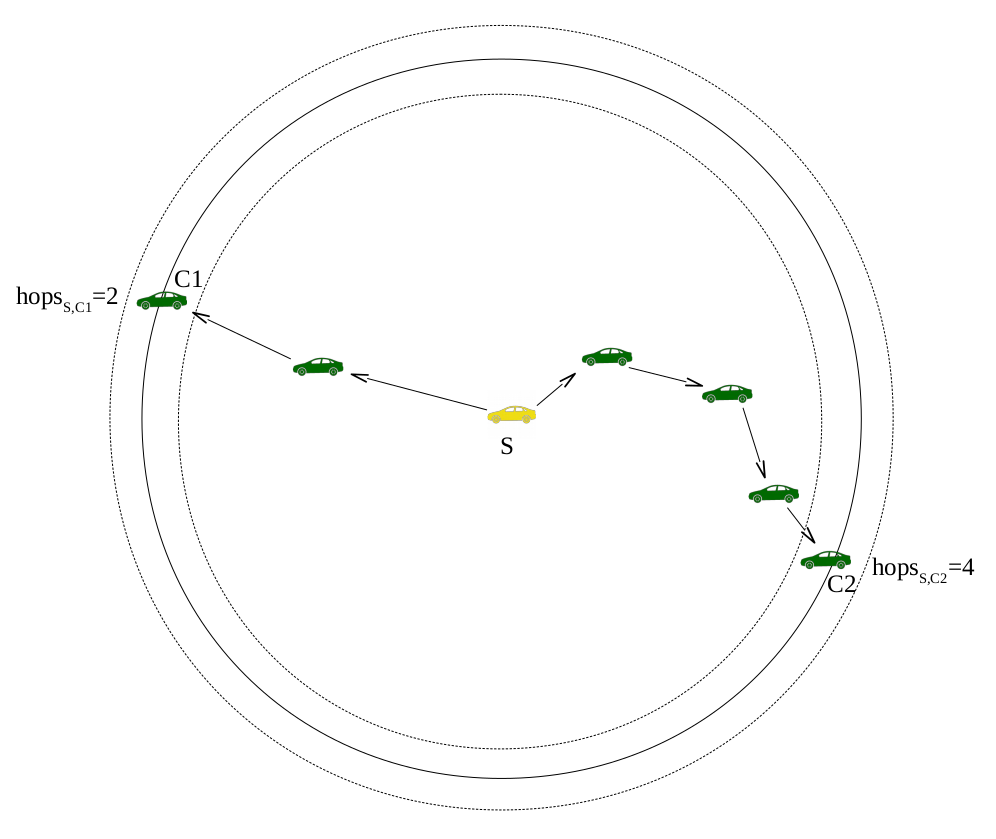
\includegraphics[width=0.7\textwidth]{immagini/hops}
				\caption{Example of \textit{NOH} calculation with Alert Message starting from node S}
				\label{fig:hops}
			\end{figure}
			
		\subsection{Number Of Slots (NOS)}
			This metric is used to measure the number of slots required in order to propagate the Alert Message from the source to all vehicles reached on the circumference. High values of this metric means that the multi-hop protocol introduces a lot of waiting time before each forwarding, hence increasing end-to-end delay and hurting the timeliness of the emergency message propagation.
		
			\begin{gather}
				\label{eq:slots}
				NOH = \frac{ \sum_{p \in RC } \textrm{\textit{no. of slots waited along path from source to p}}} {\textrm{\textit{no. of vehicles on circ}}}
			\end{gather}	
	
			where $RC$ is the set of vehicles which have successfully received the message on the circumference
			The number of slots along the path from node $a$ to $b$ at the numerator of Equation \ref{eq:slots} is the sum of the slots waited by each forwarder before relaying the Alert Message. 
			
			
			Based on the scenario represented in Figure \ref{fig:slots} and Equation \ref{eq:slots}, the mean number of slots from source S to nodes on the circumference is 100.
			
			\begin{figure}[H]
				\centering
				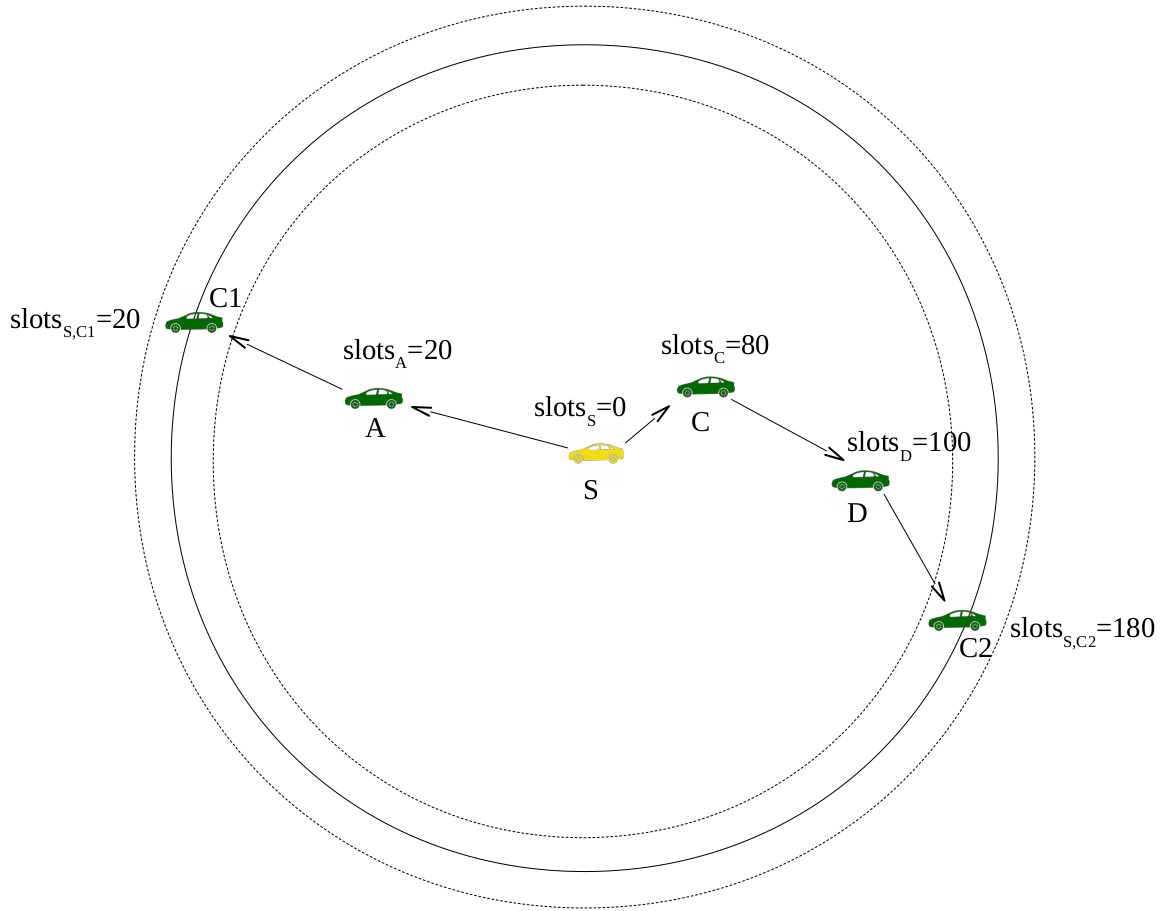
\includegraphics[width=0.7\textwidth]{immagini/slots}
				\caption{Example of \textit{NOS} calculation with Alert Message starting from node S}
				\label{fig:slots}
			\end{figure}
			
			
		\subsection{Forwarding Node Number (FNN)}
			This metric is used to measure the number of vehicles which forward the Alert Message. The value of this metric is an indicator of the effectiveness of the multi-hop protocol in successfully suppressing scheduled transmissions from PFCs after the FFC has relayed the message. The metric is calculated as follows:
			 
			\begin{gather}
				\label{eq:nos}
				FNN = \textrm{\textit{no. of vehicles forwarding the Alert Message}}
			\end{gather}	
				
	\section{Platoon scenario}
		The first scenario taken into consideration is a simple platoon scenario, where vehicles are placed in a strip-like area 15 kilometers long. Vehicles are 25 meters distant from each other. Transmission ranges of 100, 300 and 500 has been employed during simulations. 
		Parameters for this scenario are included in Table \ref{table:platoon}.  
		
		\begin{table}[H]
			\def\arraystretch{1.1}
			\rowcolors{2}{D}{P}	
			\begin{tabularx}{\textwidth}{l | l  l}
				\rowcolor{I} {\large \textcolor{white}{Parameter}} & {\large \textcolor{white}{Value}} & {\large \textcolor{white}{}} \TBstrut  \\
				\toprule
				\endhead
	%			\midrule[1pt]
				\rowcolor{P} \multicolumn{3}{c}{Scenario configuration} \\
				\midrule[1pt]
				Road length 							& 15000 				& m		\\
				Distance between vehicles 				& 25					& m		\\
				Circumference	radius					& 14000					& m		\\
				Number of vehicles						& 600					& 		\\
				Source of alert message position		& Left of platoon		&		\\
				Mobility model							& ns3::ConstantPosition	&		\\
				\midrule[1pt]
				\rowcolor{P} \multicolumn{3}{c}{Network configuration} \\
				\midrule[1pt]
				Packet size								& 100					& byte	\\	
				Transmission standard					& 802.11b				&		\\
				Frequency								& 2.4					& GHz	\\
				Channel bandwidth						& 22					& MHz	\\
				Transmission speed						& 11					& Mbps	\\
				Transmission powers						& -7.0, 4.6, 13.4		& dBm	\\
				Transmission range						& 100, 300, 500			& m		\\
				Modulation								& DSSS					& 		\\
				Propagation loss model					& ns3::TwoRayGround 	&		\\
				Shadowing model							& No					&		\\
				Propagation delay model					& ns3::ConstantSpeed	&		\\
				Junction modeling						& No					&		\\
				\midrule[1pt]
				\rowcolor{P} \multicolumn{3}{c}{Protocols configuration} \\
				\midrule[1pt]
	%			Protocols tested						& \makecell{FB, ROFF, STATIC100, \\ STATIC300, STATIC500} & \\
				FB contention window					& [32, 1024]			& slot	\\
				ROFF distance range (\textit{k} parameter) & 1					&		\\	
				\midrule[1pt]
				Number of simulations per configuration	& 1000					&		\\
				\bottomrule
			\end{tabularx}
			\label{table:platoon}
			\caption{Platoon scenario configuration}
		\end{table}
	
		\begin{figure}[H]
			\centering
			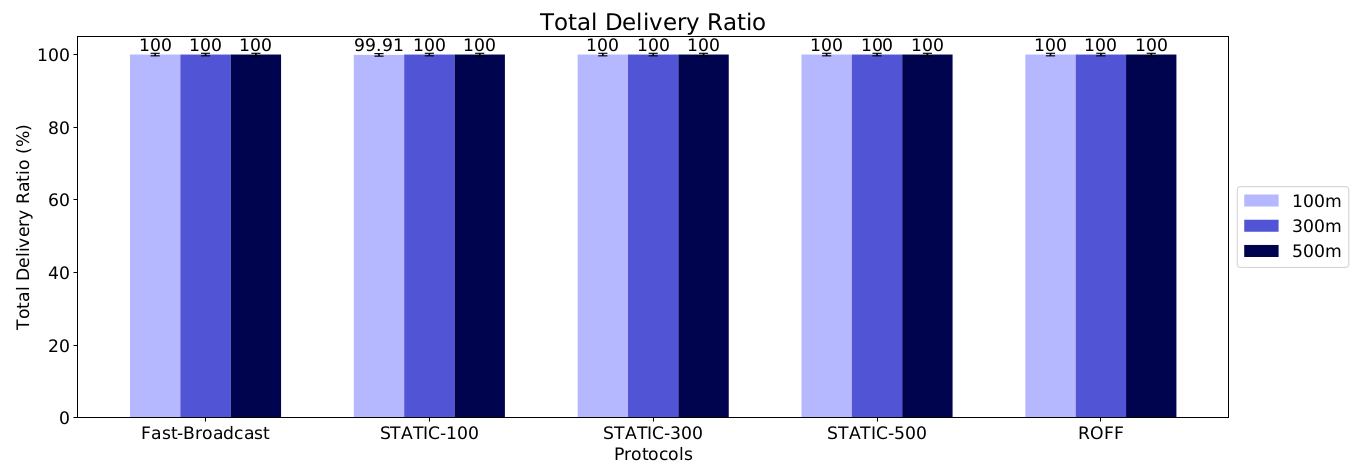
\includegraphics[width=1.1\textwidth]{immagini/platoon-15km/tdr}
			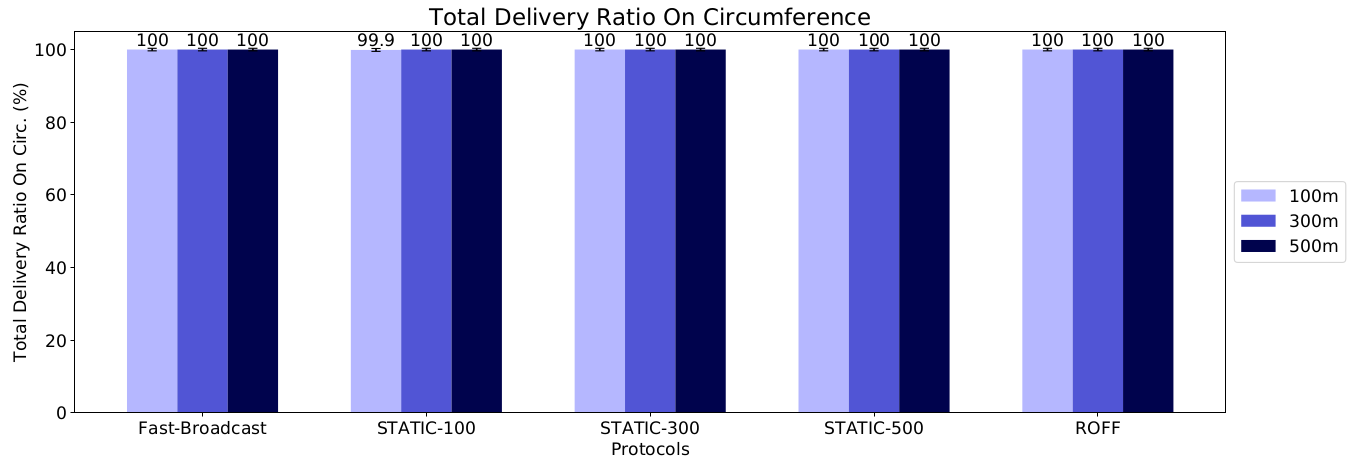
\includegraphics[width=1.1\textwidth]{immagini/platoon-15km/tdroc}
			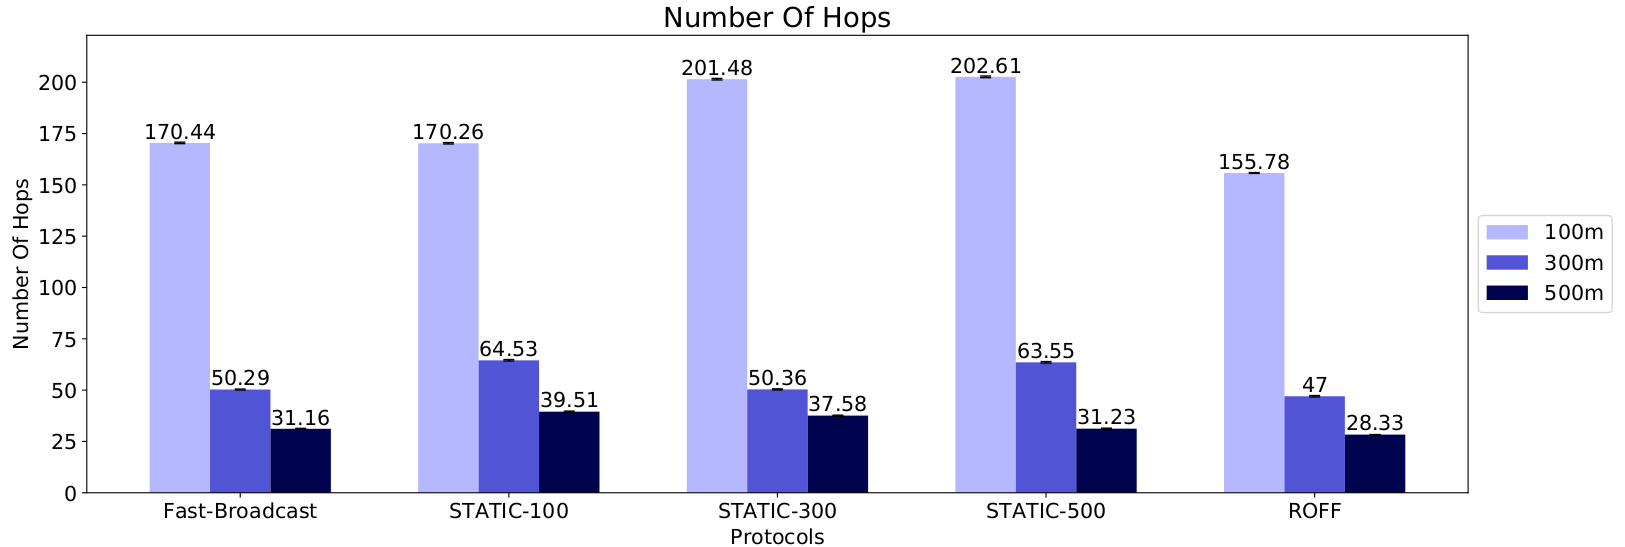
\includegraphics[width=1.1\textwidth]{immagini/platoon-15km/noh}
			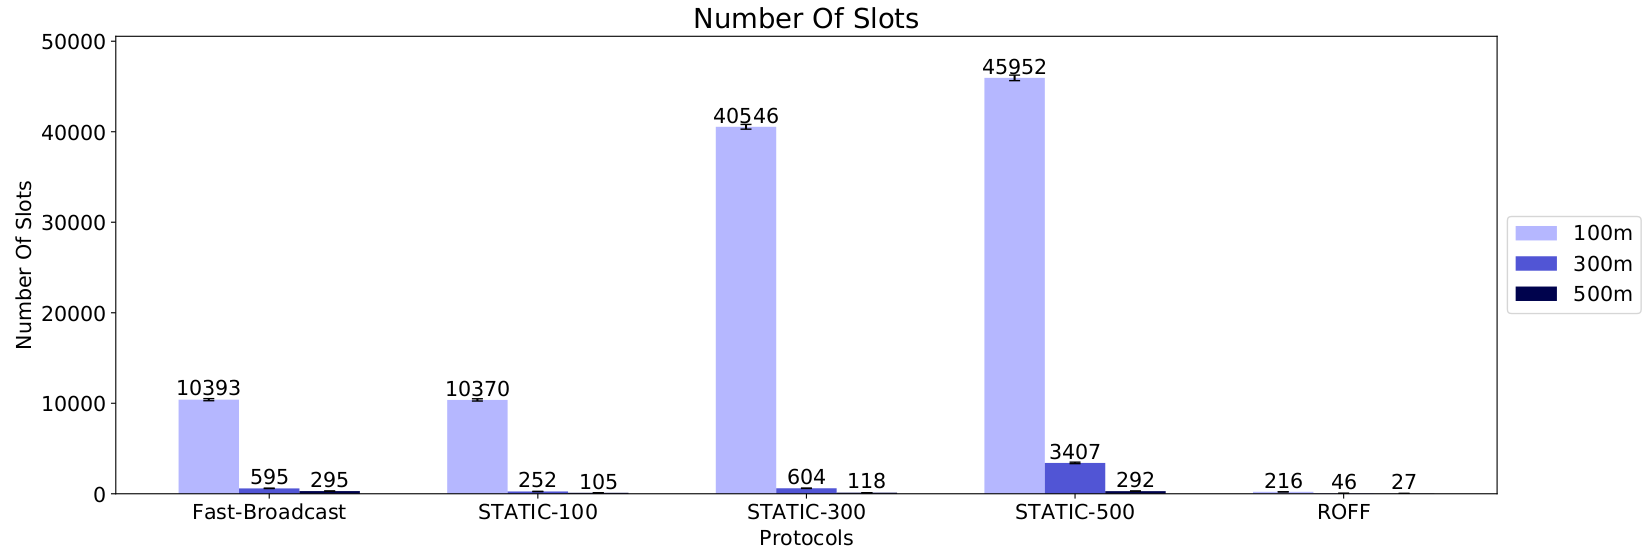
\includegraphics[width=1.1\textwidth]{immagini/platoon-15km/nos}
			\caption{\textit{TDR}, \textit{TDROC}, \textit{NOH} and \textit{NOS} metrics for Platoon scenario}
			\label{fig:metric-platoon-15km-1}
		\end{figure}

		\begin{figure}[H]
			\centering
			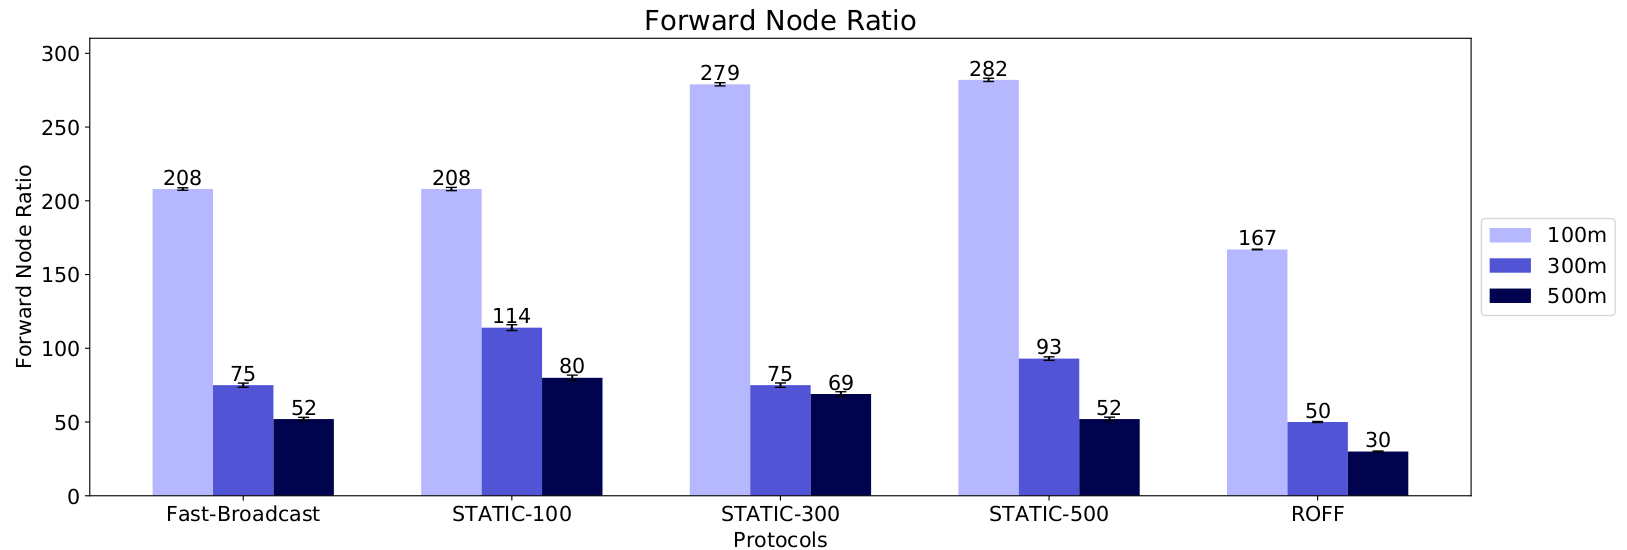
\includegraphics[width=1.1\textwidth]{immagini/platoon-15km/fnn}
			\caption{\textit{FNN} metric for Platoon scenario }
			\label{fig:metric-platoon-15km-2}
		\end{figure}
	
		Since this scenario is one-dimensional, the circumference simply consists in vehicles distant $14.000  \pm 12$ meters from the source of Alert Message. Both metrics about Delivery Ratio (global and on circumference) are close to 100\%, so the algorithms successfully propagate the AM until the end of the platoon.
		
		
		Considering the Number Of Hops, ROFF's results are 11,76\%, 6,54\% and 9,08\% lower than Fast-Broadcast's results respectively for 100, 300 and 500 meters transmission range. ROFF's results are close to the optimal number of hops, respectively 140, 46,6 and 28 for the same transmission ranges as above. This means that the forwarder selection algorithms based on ESD Bitmap works better in choosing the farthest vehicle from the previous forwarder compared to the contention window approach for 1D scenarios. Considering STATIC variants of Fast-Broadcast, it is possible to observe that the STATIC-tx variant produces comparable results with Fast-Broadcast with \textit{tx} transmission range (e.g. STATIC-100 value is comparable to Fast-Broadcast with 100 meters transmission range), as expected. The STATIC protocol performs worse (hence the Number of Hops increases) whenever the transmission range is underestimated (e.g. STATIC-100 with 300 meters transmission range, compared to Fast-Broadcast with the same transmission range) or overestimated (e.g. STATIC-500 with 100 meters transmission range, compared to Fast-Broadcast with the same transmission range). This behaviour is expected, as reported in \cite{BAR2017}.
		
		
		Regarding the Number of Slots, ROFF's performs much better than Fast-Broadcast. The metric's value is decreased respectively by 97,92\%, 92,27\% and 90,85\%  using ROFF. The waiting time calculation, based on unique forwarding priority instead of distance, guarantees a much lower wait compared to Fast-Broadcast contention window approach. As before, STATIC approaches produce results comparable with Fast-Broadcast when the transmission range estimation is correct. Instead, the Number of Slots greatly increases when the transmission range is underestimated and decreases when the transmission range is overestimated. In this last case, the decrease in NOS comes with an increase in Number Of Hops reported in the previous paragraph, so an overestimation of transmission range is not desirable.
		
		
		Lastly, it is possible to see that ROFF's achieves a better suppression of redundant transmissions, guaranteeing a decrease of 19,71\%, 33,33\% and 42,31\$ respectively for each one of the transmission ranges considered.
		
		
	\section{Grid scenario}
		After tests on the 1D Platoon scenario have been carried out, the next step consisted in testing the algorithms' performances in a 2D Grid scenario, employing also the shadowing model introduced in \ref{sec:shadowing}.
		Parameters for this scenario are included in Table \ref{tab:grid}.  
		
		\begin{table}[H]
			\def\arraystretch{1.1}
			\rowcolors{2}{D}{P}	
			\begin{tabularx}{\textwidth}{l | l  l}
				\rowcolor{I} {\large \textcolor{white}{Parameter}} & {\large \textcolor{white}{Value}} & {\large \textcolor{white}{}} \TBstrut  \\
				\toprule
				\endhead
				%			\midrule[1pt]
				\rowcolor{P} \multicolumn{3}{c}{Scenario configuration} \\
				\midrule[1pt]
				Road length 							& 4800	 				& m		\\
				Distance between roads					& 300					& m		\\
				Road width								& 10					& m		\\
				Number of roads (vertical)				& 17					&		\\
				Number of roads (horizontal)			& 17					&		\\
				Distance between vehicles 				& 25					& m		\\
				Circumference radius					& 2000					& m		\\
				Number of vehicles						& 6528					& 		\\
				Source of alert message position		& Center				&		\\
				Mobility model							& ns3::ConstantPosition	&		\\
				Edge of buildings						& 290					& m		\\
				Number of buildings						& 255					& m		\\
				\midrule[1pt]
				\rowcolor{P} \multicolumn{3}{c}{Network configuration} \\
				\midrule[1pt]
				Shadowing model							& Obstacle Shadowing	&		\\
				Junction modeling						& No					&		\\
				\midrule[1pt]
				Number of simulations per configuration	& 1000					&		\\
				\bottomrule
			\end{tabularx}
			\caption{Grid scenario configuration}
			\label{tab:grid}
		\end{table}
	
		\begin{figure}[H]
			\centering
			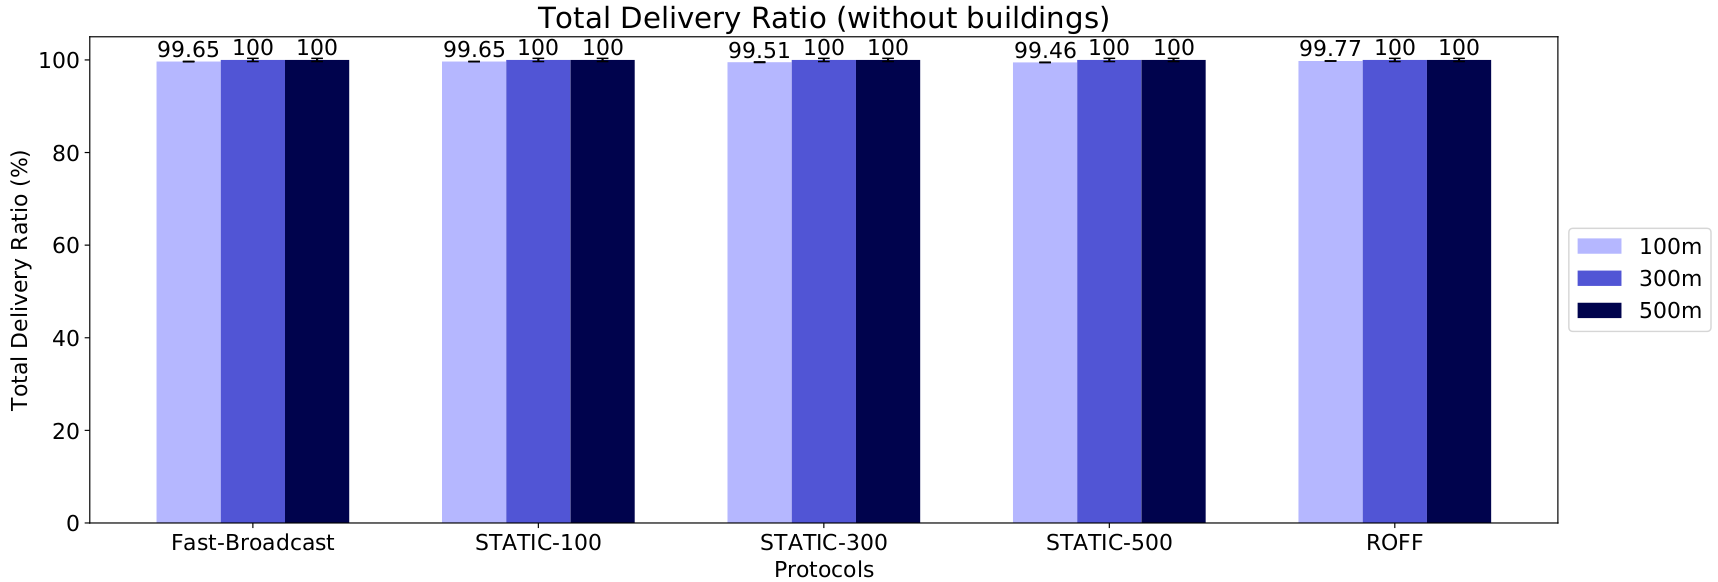
\includegraphics[width=1.0\textwidth]{immagini/grid-300/b0/tdr}
			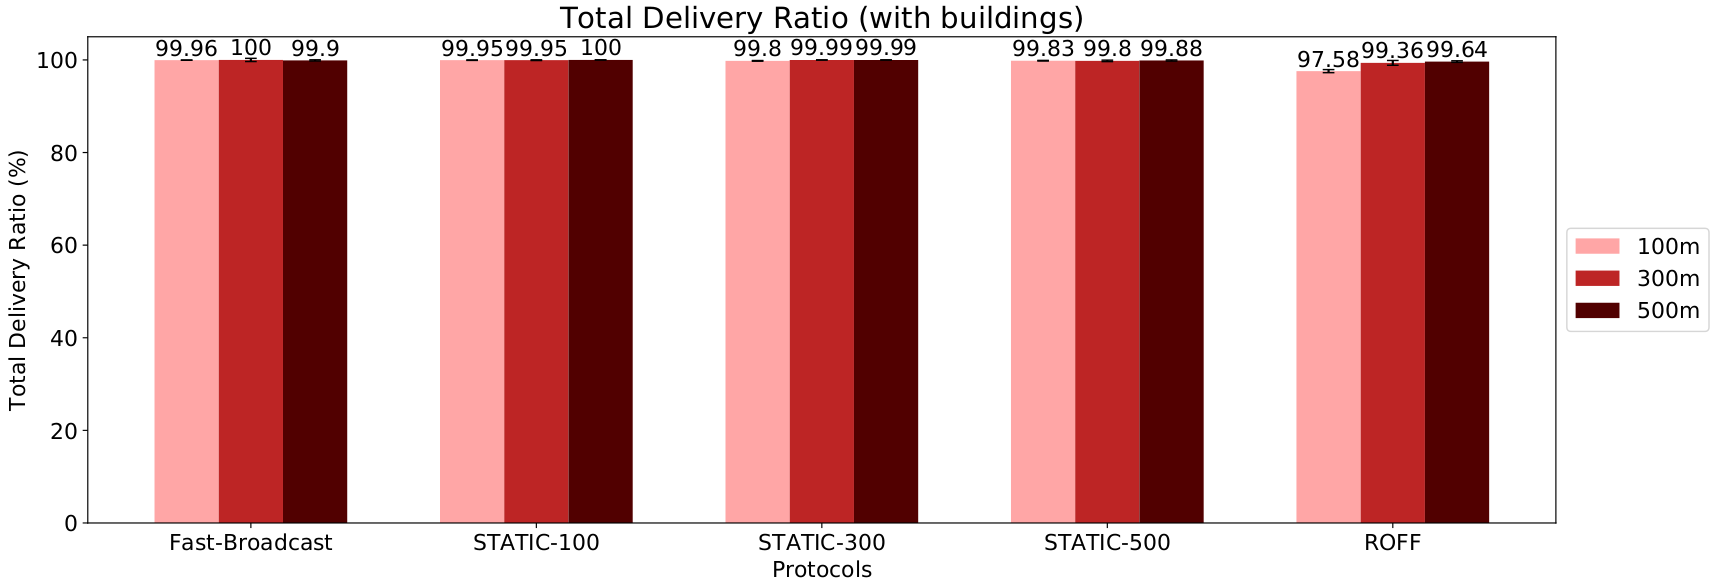
\includegraphics[width=1.0\textwidth]{immagini/grid-300/b1/tdr}
			\caption{\textit{TDR} without buildings (top) and with buildings (bottom) for Grid scenario}
			\label{fig:grid-tdr}
		\end{figure}
		
		\begin{figure}[H]
			\centering
			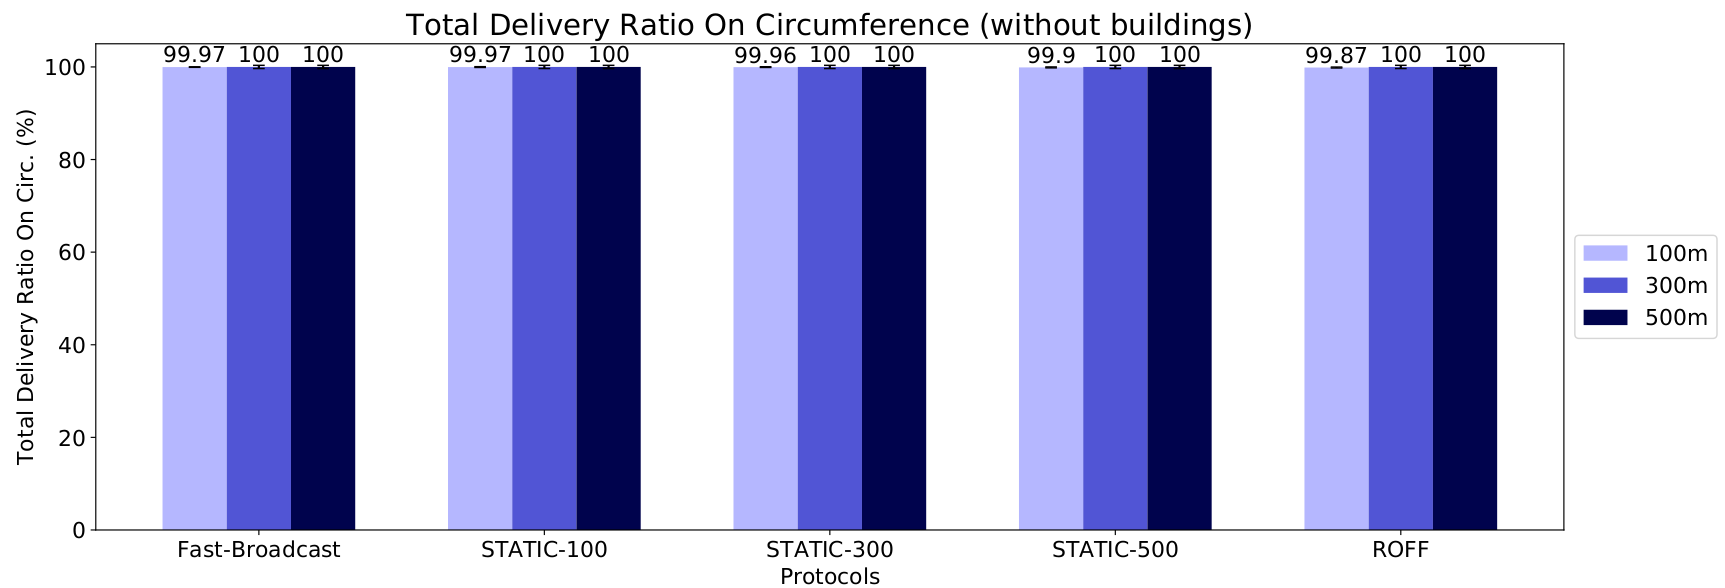
\includegraphics[width=1.0\textwidth]{immagini/grid-300/b0/tdroc}
			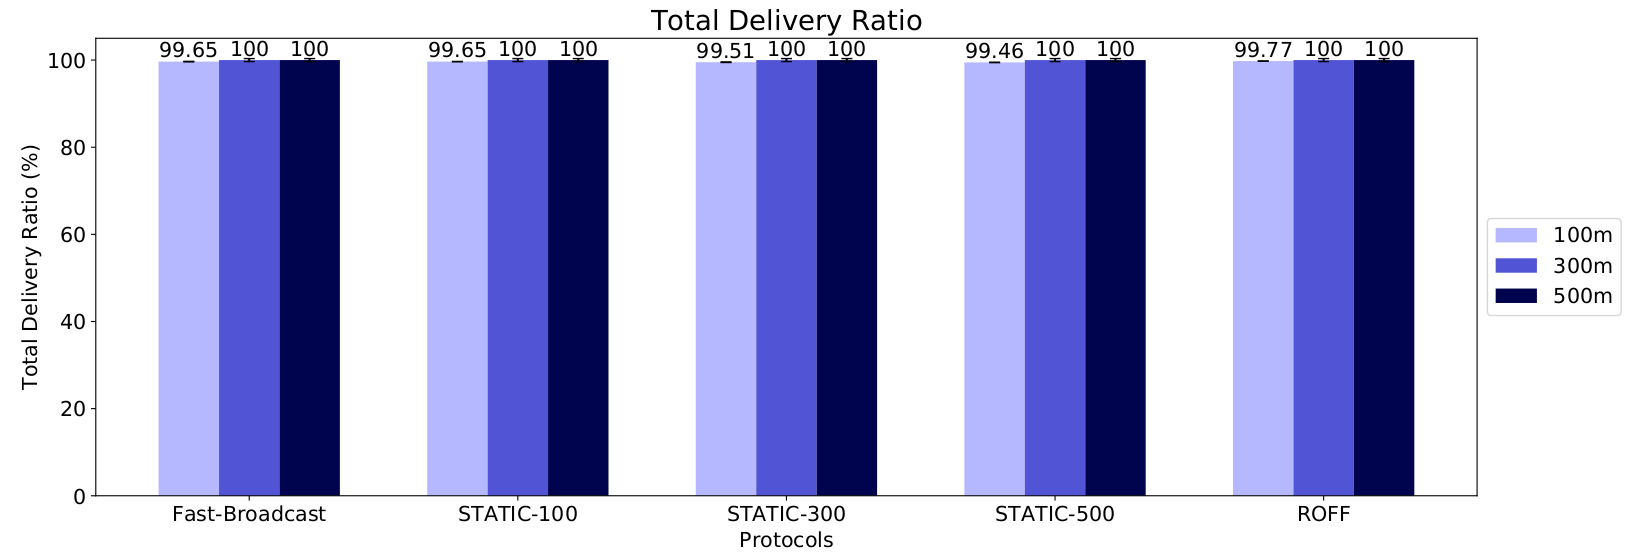
\includegraphics[width=1.0\textwidth]{immagini/grid-300/b1/tdroc}
			\caption{\textit{TDROC} without buildings (top) and with buildings (bottom) for Grid scenario}
			\label{fig:grid-tdroc}
		\end{figure}
	
		\begin{figure}[H]
			\centering
			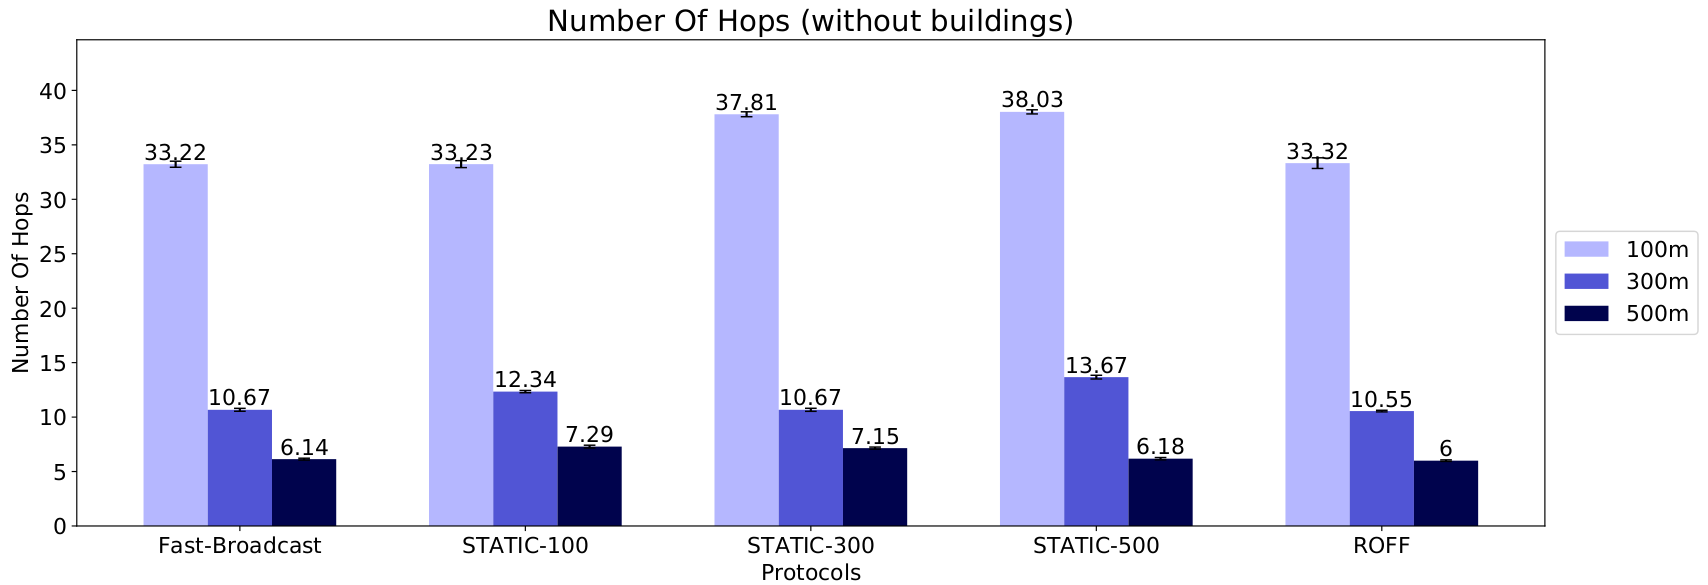
\includegraphics[width=1.0\textwidth]{immagini/grid-300/b0/noh}
			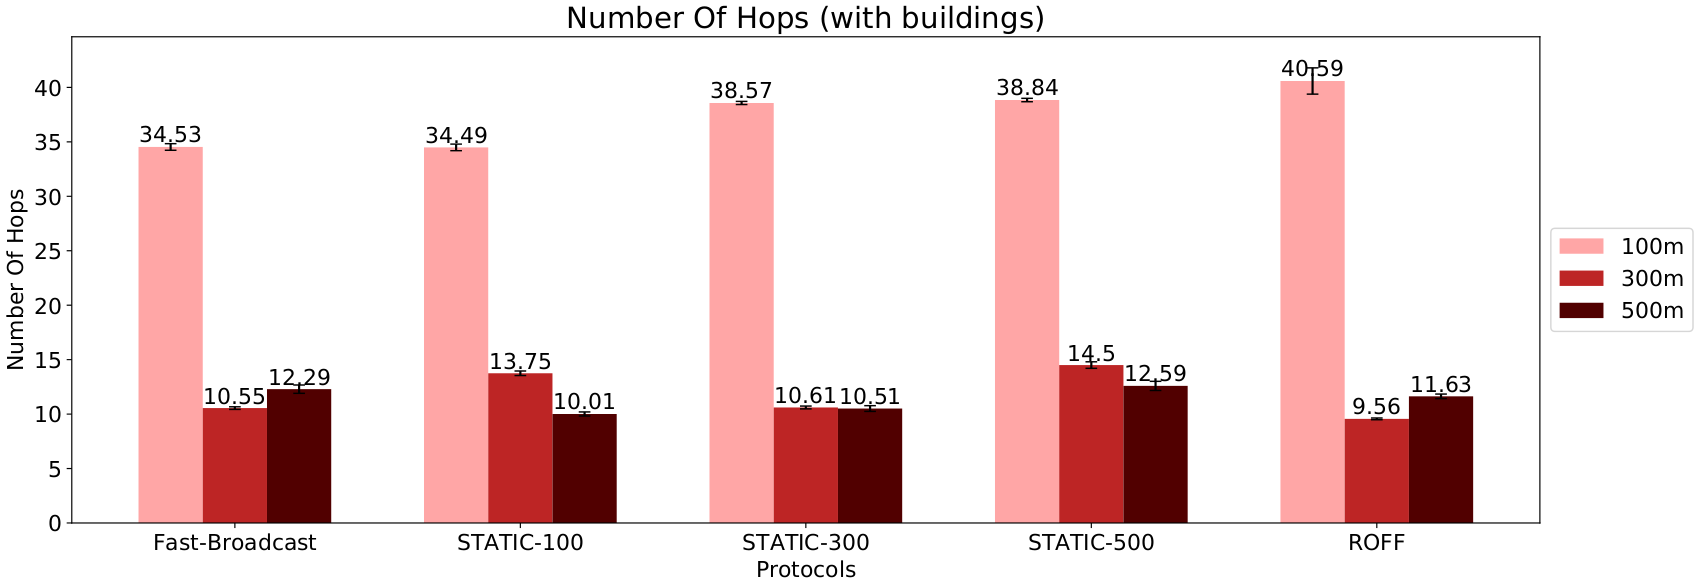
\includegraphics[width=1.0\textwidth]{immagini/grid-300/b1/noh}
			\caption{\textit{NOH} without buildings (top) and with buildings (bottom) for Grid scenario}
			\label{fig:grid-noh}
		\end{figure}
	
		\begin{figure}[H]
			\centering
			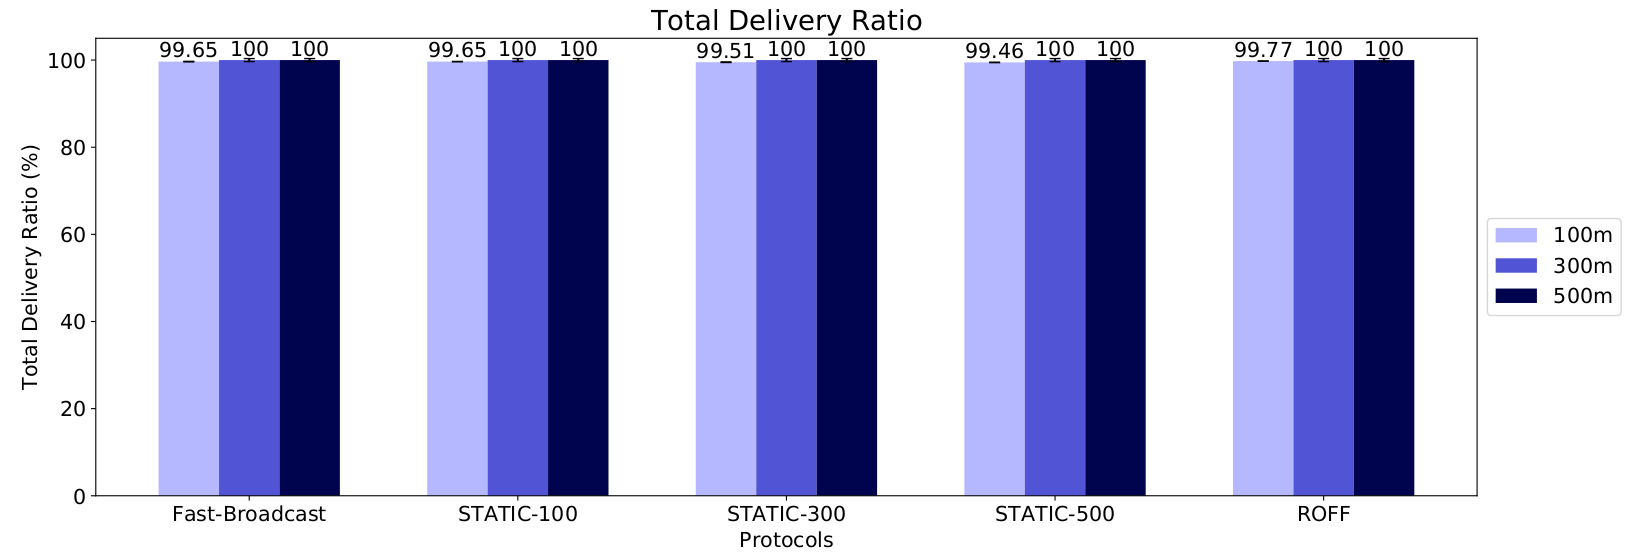
\includegraphics[width=1.0\textwidth]{immagini/grid-300/b0/nos}
			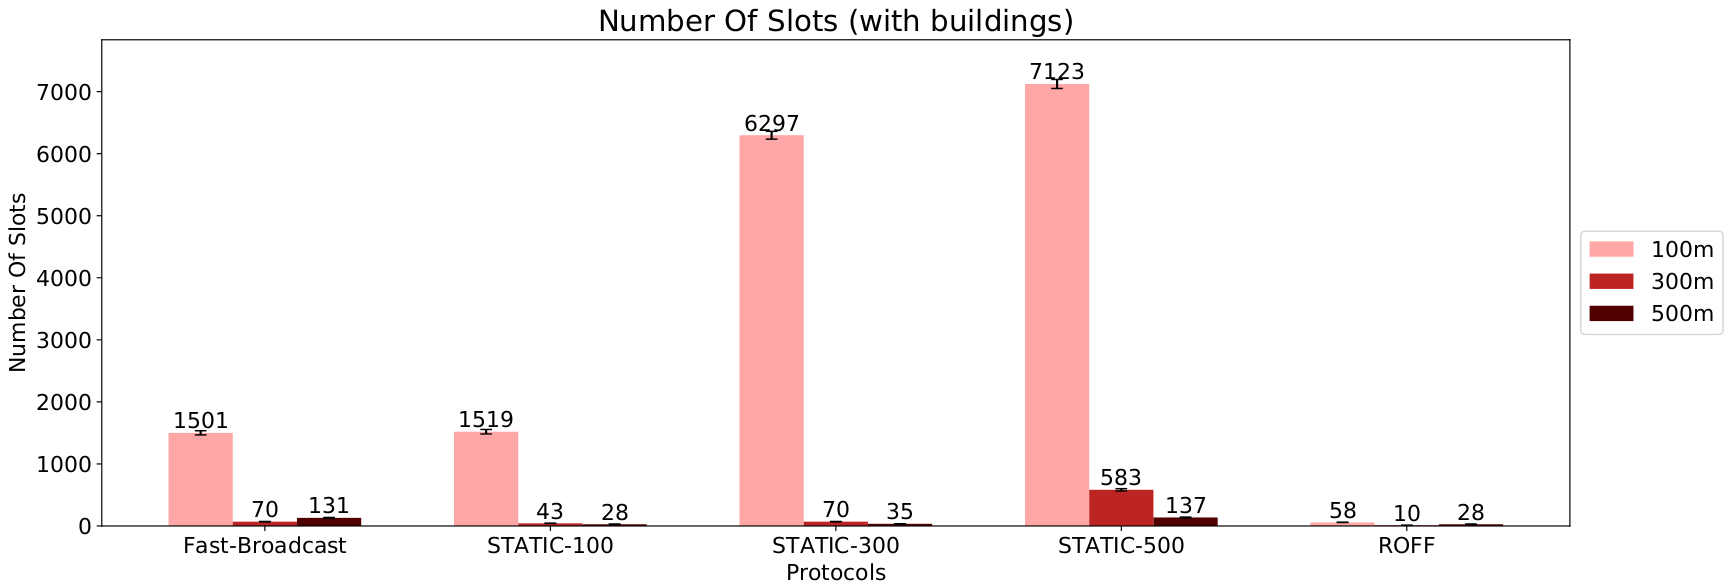
\includegraphics[width=1.0\textwidth]{immagini/grid-300/b1/nos}
			\caption{\textit{NOS} without buildings (top) and with buildings (bottom) for Grid scenario}
			\label{fig:grid-nos}
		\end{figure}
	
		\begin{figure}[H]
			\centering
			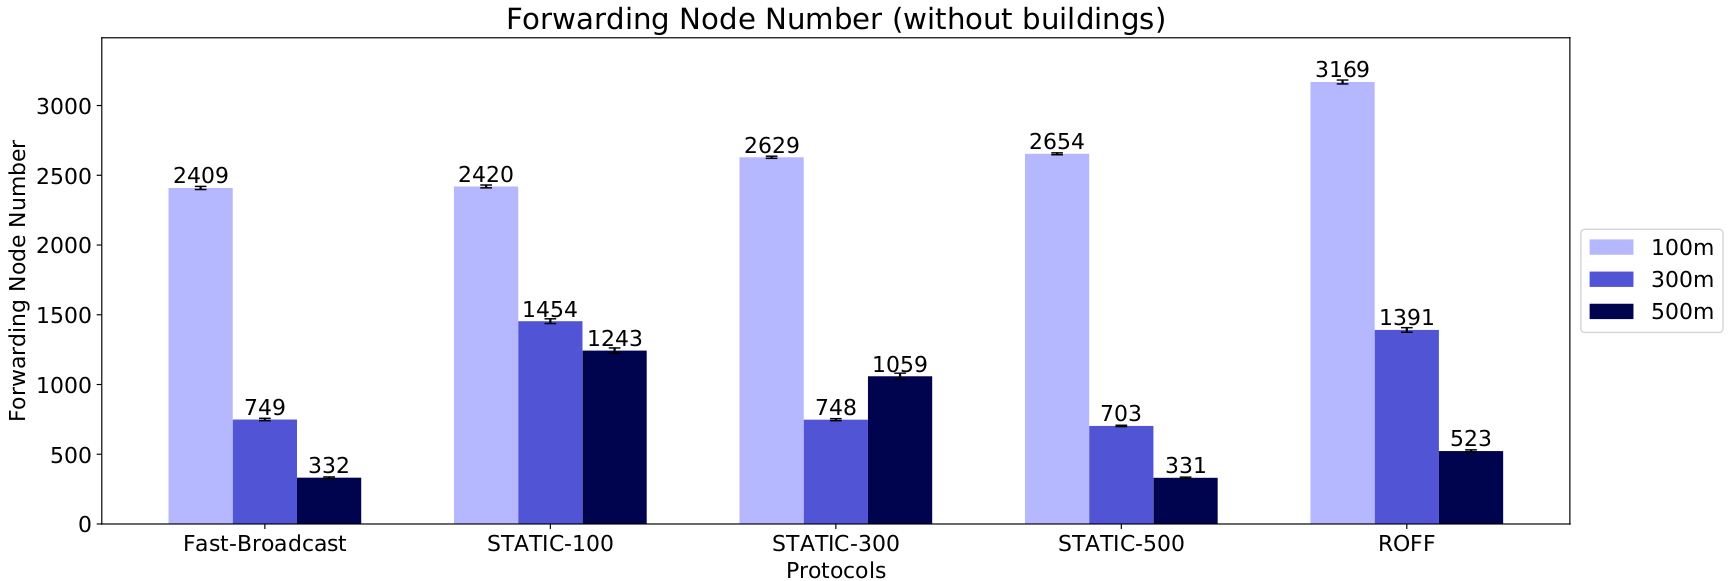
\includegraphics[width=1.0\textwidth]{immagini/grid-300/b0/fnn}
			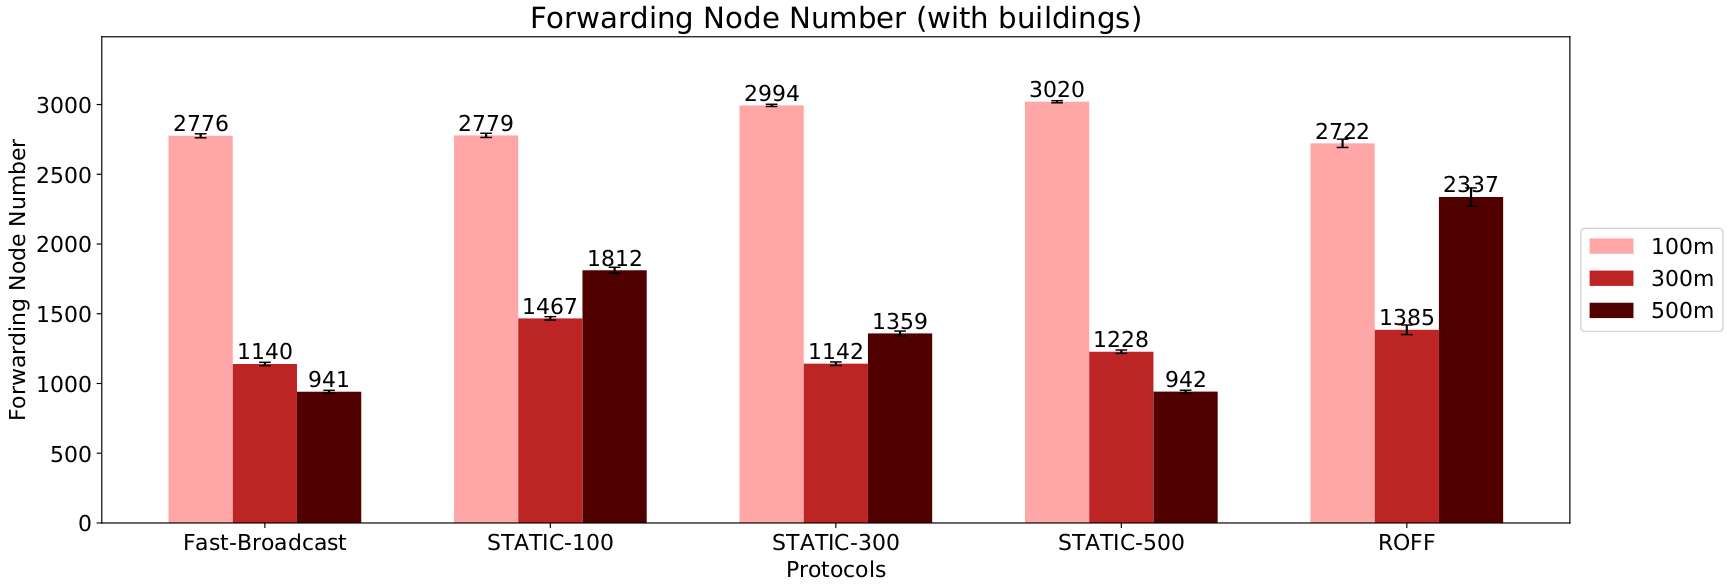
\includegraphics[width=1.0\textwidth]{immagini/grid-300/b1/fnn}
			\caption{\textit{FNN} without buildings (top) and with buildings (bottom) for Grid scenario}
			\label{fig:grid-fnn}
		\end{figure}
	
		All the algorithms perform well as far as delivery ratios are concerned (Figure \ref{fig:grid-tdr} \ref{fig:grid-tdroc}), both for scenarios with and without buildings. This means that the shadowing caused by the Obstacle Model does not create no-reach zones, and the signal manages to find its way to almost all of the vehicles. The regular pattern by which vehicles are placed may help with that: further testing where this hypothesis is removed will be presented in the next sections. Even though delivery ratios are unchanged, the effect of the Obstacle model can be observed qualitatively comparing Figure \ref{fig:fb-b0-grid-transmission} and \ref{fig:fb-b1-grid-transmission} for Fast-Broadcast, and Figure \ref{fig:roff-b0-grid-transmission} and \ref{fig:roff-b1-grid-transmission} for ROFF. The effects of obstacles on propagation cause the signal to travel only through roads segments where line of sight is possible. Instead, without obstacles the signal can be propagated freely in all directions.
		
		
		Moreover, Fast-Broadcast and ROFF can be compared with each other by looking at Figure \ref{fig:fb-b0-grid-transmission} and \ref{fig:roff-b0-grid-transmission} for the scenario without buildings, and Figure \ref{fig:fb-b1-grid-transmission} and \ref{fig:roff-b1-grid-transmission} for the scenario with buildings. In both cases, ROFF designates the furthest PFC as the next forwarder much more reliably than Fast-Broadcast thanks to the Neighbor Table mechanism. Instead, Fast-Broadcast relies on a random choice of waiting time, so the next designated forwarder is sometimes not one of the farthest vehicles from the previous forwarder. Based on this observation, we can expect a much lower NOH value for ROFF. Quantitative analysis of this and other metrics will be reported in the next paragraphs of this section.
		
		\begin{figure}[H]
			\centering
			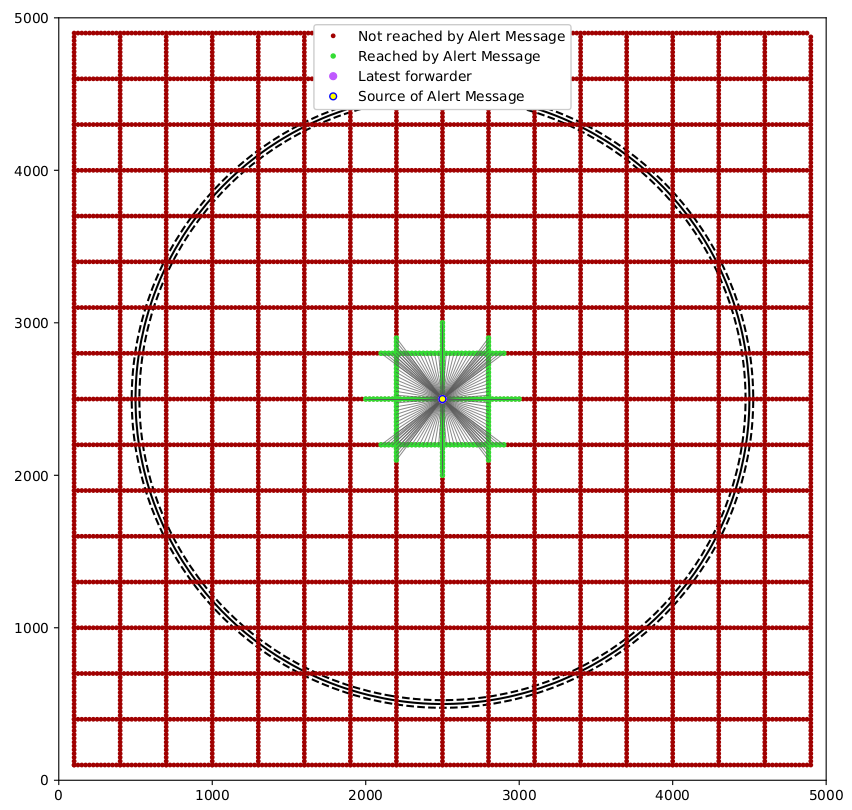
\includegraphics[width=0.8\textwidth]{immagini/grid-300/b0/fb-1hop}
			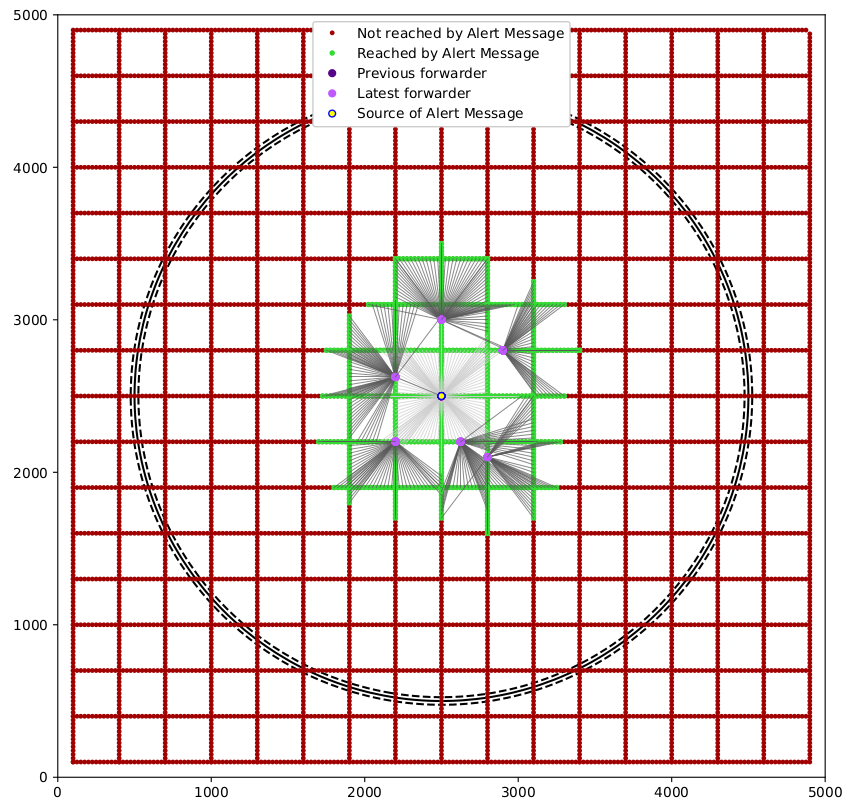
\includegraphics[width=0.8\textwidth]{immagini/grid-300/b0/fb-2hop}
			\caption{Fast-Broadcast after 1 hop (top) and 2 hops (bottom) in Grid scenario with 500 meters transmission range and without the Obstacle model}
			\label{fig:fb-b0-grid-transmission} 
		\end{figure}
		
		\begin{figure}[H]
			\centering
			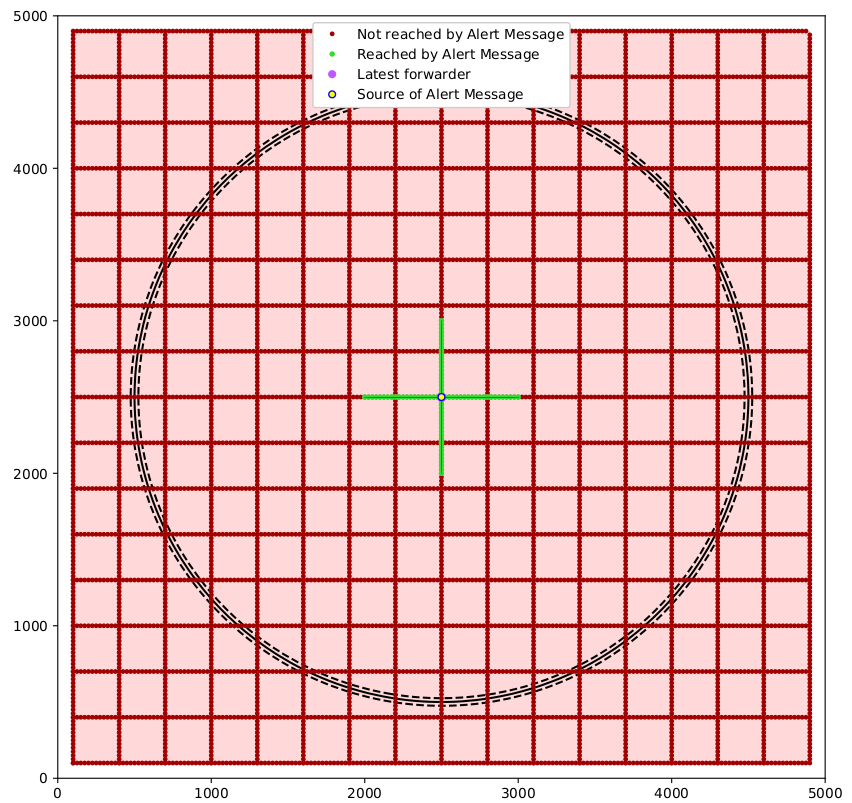
\includegraphics[width=0.8\textwidth]{immagini/grid-300/b1/fb-1hop}
			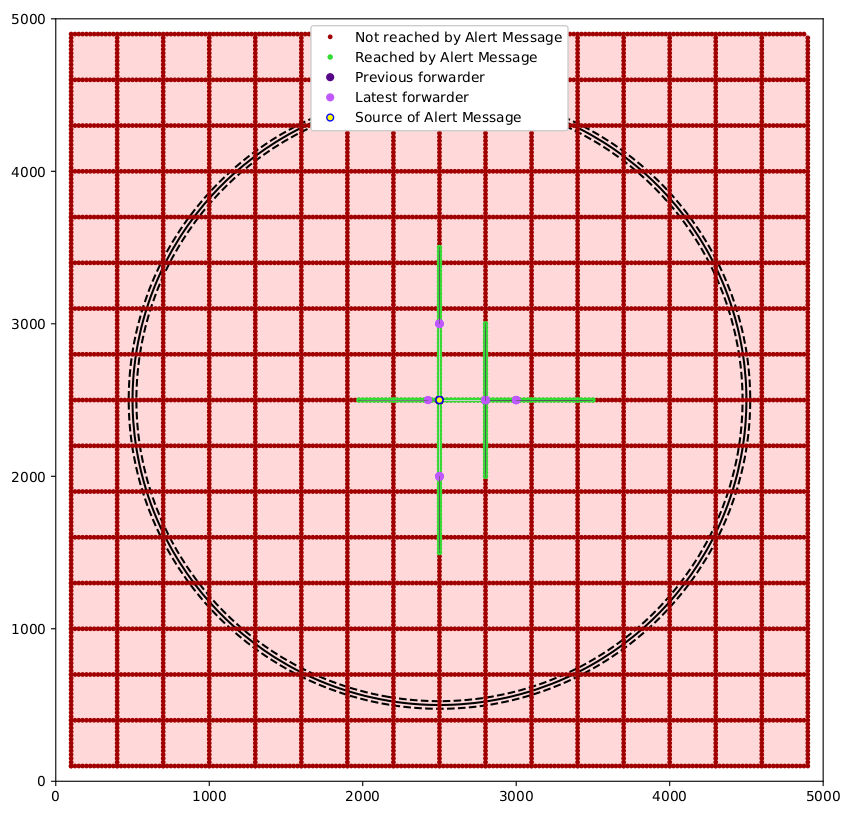
\includegraphics[width=0.8\textwidth]{immagini/grid-300/b1/fb-2hop}
			\caption{Fast-Broadcast after 1 hop (top) and 2 hops (bottom) in Grid scenario with 500 meters transmission range and with the Obstacle model}
			\label{fig:fb-b1-grid-transmission} 
		\end{figure}
	
		\begin{figure}[H]
			\centering
			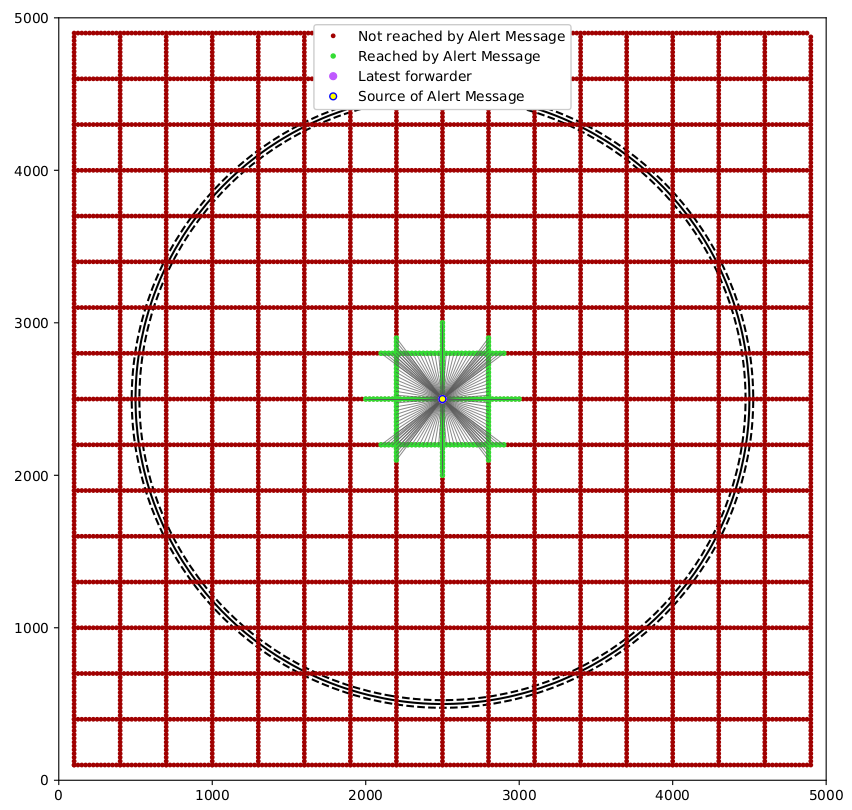
\includegraphics[width=0.8\textwidth]{immagini/grid-300/b0/fb-1hop}
			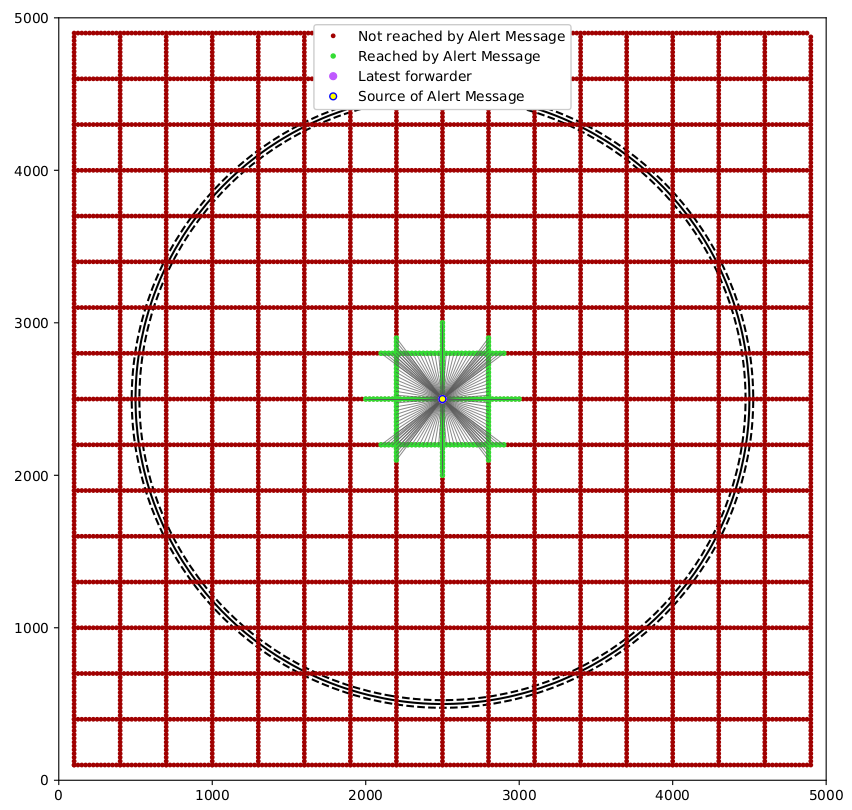
\includegraphics[width=0.8\textwidth]{immagini/grid-300/b0/fb-1hop}
			\caption{ROFF after 1 hop (top) and 2 hops (bottom) in Grid scenario with 500 meters transmission range and without the Obstacle model}
			\label{fig:roff-b0-grid-transmission} %todo
		\end{figure}
	
		\begin{figure}[H]
			\centering
			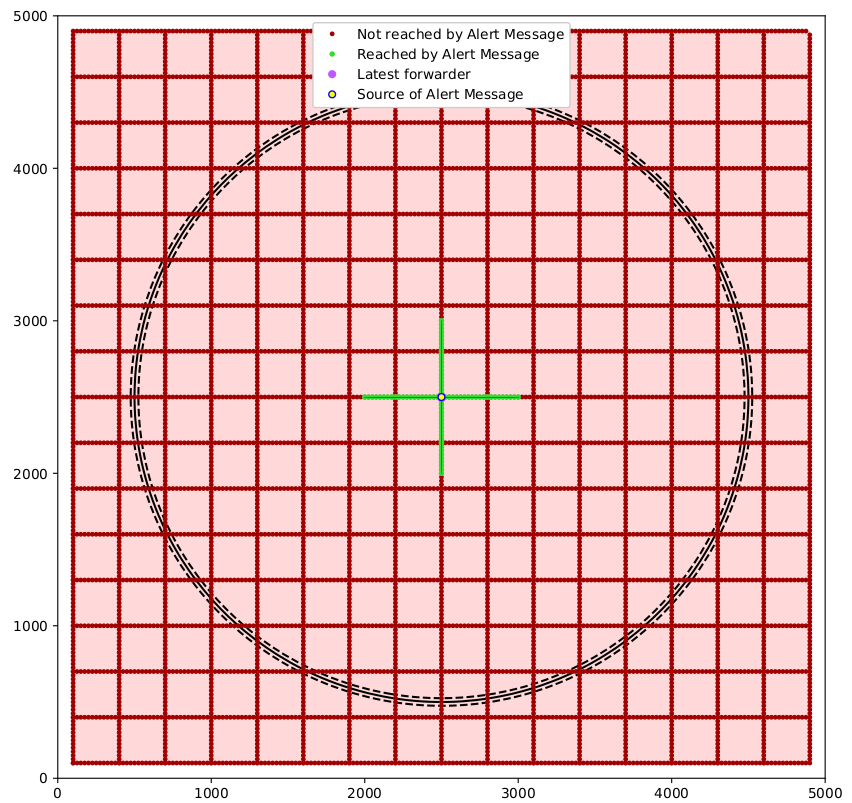
\includegraphics[width=0.8\textwidth]{immagini/grid-300/b1/fb-1hop}
			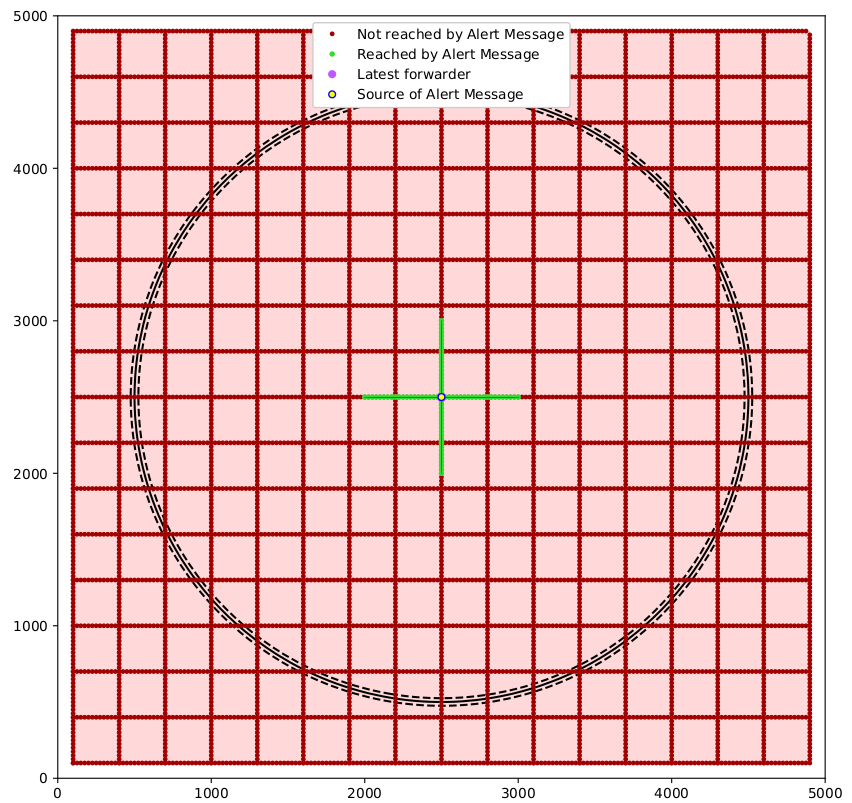
\includegraphics[width=0.8\textwidth]{immagini/grid-300/b1/fb-1hop}
			\caption{ROFF after 1 hop (top) and 2 hops (bottom) in Grid scenario with 500 meters transmission range and with the Obstacle model}
			\label{fig:roff-b1-grid-transmission} %todo
		\end{figure}
		
		If we focus on the Number Of Hops (Figure \ref{fig:grid-noh}), we notice that the introduction of buildings causes the number of hops to increases for transmission ranges of 100 and 500 meters, while decreases for 300 meters tranmission range. This is probably due to the fact that the distance between roads is also 300 meters and the starting vehicle is inside a junction. This means that the effect of buildings causes the signal to travel along roads, hopping from junction to junction, and reaching the circumference much faster. Another unusual observervation consists in ROFF with 100 meters transmission range, where the value increases by a lot. This case needs further examination in order to be explained. Apart from this case, ROFF achieves better results than Fast-Broadcast, with results 9\% and 3.47\% better for 300 and 500 meters transmission range respectively. 
		
		
		The analysis of the Number Of Slots (Figure \ref{fig:grid-nos}) shows similar results: the shadowing model causes the metric's value to rise in all configurations except for ROFF with 300 meters transmission range. ROFF continues to outperform Fast-Broadcast with results similar to those observed in the Platoon scenario. 
		
		
		Considering the Forwarding Node Number (Figure \ref{fig:grid-fnn}), the situation is much different than the previous scenario. It is possible to see in both graphs that ROFF's values are higher than Fast-Broadcast's across all configurations. Despite the almost-perfect suppression of redundant transmission works in a 1D scenario, as observer in the previous section, the mechanism does not seem to have much of an effect in a 2D scenario, regardless of the presence of buildings. A possible explanation of this phenomenon might be the one reported in Figure \ref{fig:2d-roff}, which indicates a possible Alert Message propagation process. Suppose that S is the previous forwarder: the other nodes on the circumference (distant txRange from S) are the elected FFCs which win the contention and relay the message. Due to how ROFF works, those nodes send the message at the same time, hence if we focus on A and B we have a collision area (the red area in Figure \ref{fig:2d-roff}). The nodes inside that collision area receive the forwarding from A and B at the same time and a collision occurs. As a consequence, they are not aware that the message has already been forwarded and some of them will fire their transmission. This process is repeated for every forward (and also for other FFCs other than A and B in the example) and so this could cause the increase in the FNN value. In other words, ROFF is guaranteed to cause the collision area shown in the example due to the exact waiting time calculation for nodes at the same distance from S. Fast-Broadcast is less affected by this problem since the waiting time calculation is not deterministic (the waiting time is chosen randomly from the interval [1...CW] where CW is calculated using Formula \ref{eq:contention-window}).
	
		\begin{figure}[H]
			\centering
			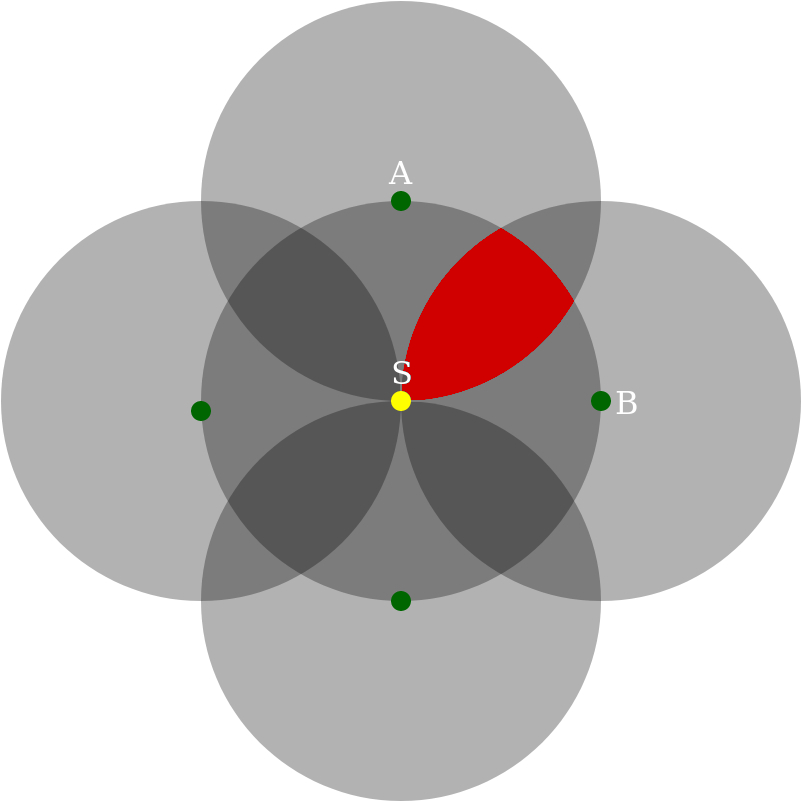
\includegraphics[width=0.5\textwidth]{immagini/2d-roff}
			\caption{Collision area in 2D ROFF}
			\label{fig:2d-roff}
		\end{figure}

	\section{Los Angeles urban scenario}
		\label{sec:la-scenario}
		The next step consisted in expanding the 2D scenario with realistic urban data taken from OpenStreetMap and processed by SUMO as explained in Section \ref{sec:sumo}. In addition to the shadowing model, in this scenario (and also in the urban scenario regarding Padua, which will be presented in the next section), a \textit{smart junction} variant of the algorithms has been introduced in order to try to increase the delivery ratios. 
		
		Figure \ref{fig:la-scenario} depicts the scenario with vehicles (green dots), buildings (purple polygons) and junctions (yellow polygons).
		
		
		All configurations are reported in Figure \ref{fig:la-overview}. In order to facilitate the understanding of the various configurations, the following graphs will utilize shades of color similar to those in Figure \ref{fig:la-overview} (e.g. graphs with shades of blue will represent a scenario without buildings and without junctions, while shades of orange will represent a scenario with buildings and with junctions). Parameters for this scenario are included in Table \ref{tab:la-25}.  
		
		\begin{figure}[H]
			\centering
			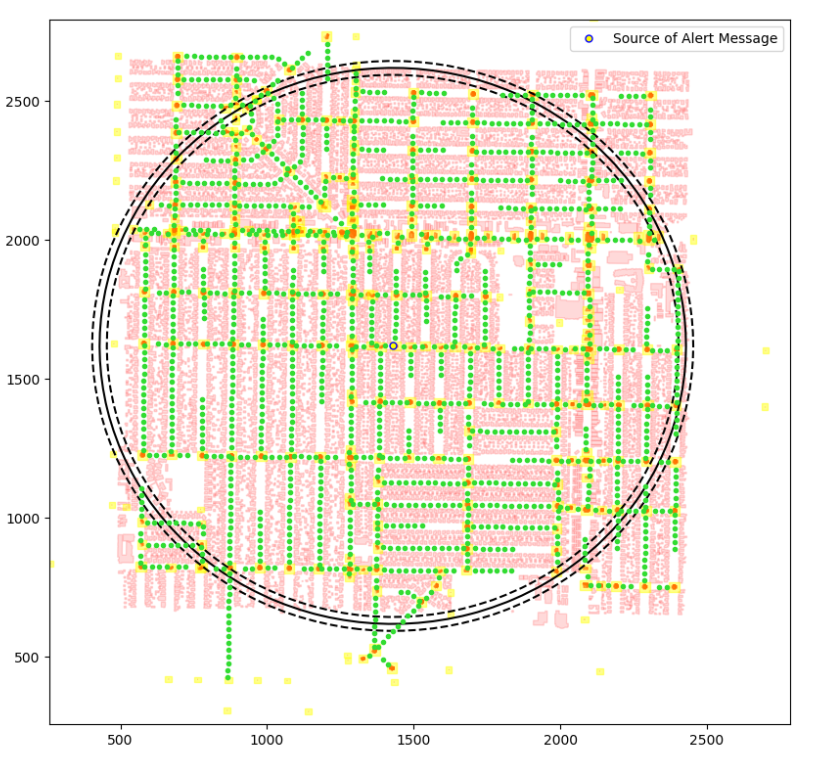
\includegraphics[width=1.0\textwidth]{immagini/la-25/la-scenario}
			\caption{Los Angeles urban scenario depiction}
			\label{fig:la-scenario}
		\end{figure}
		
		\begin{figure}[H]
			\centering
			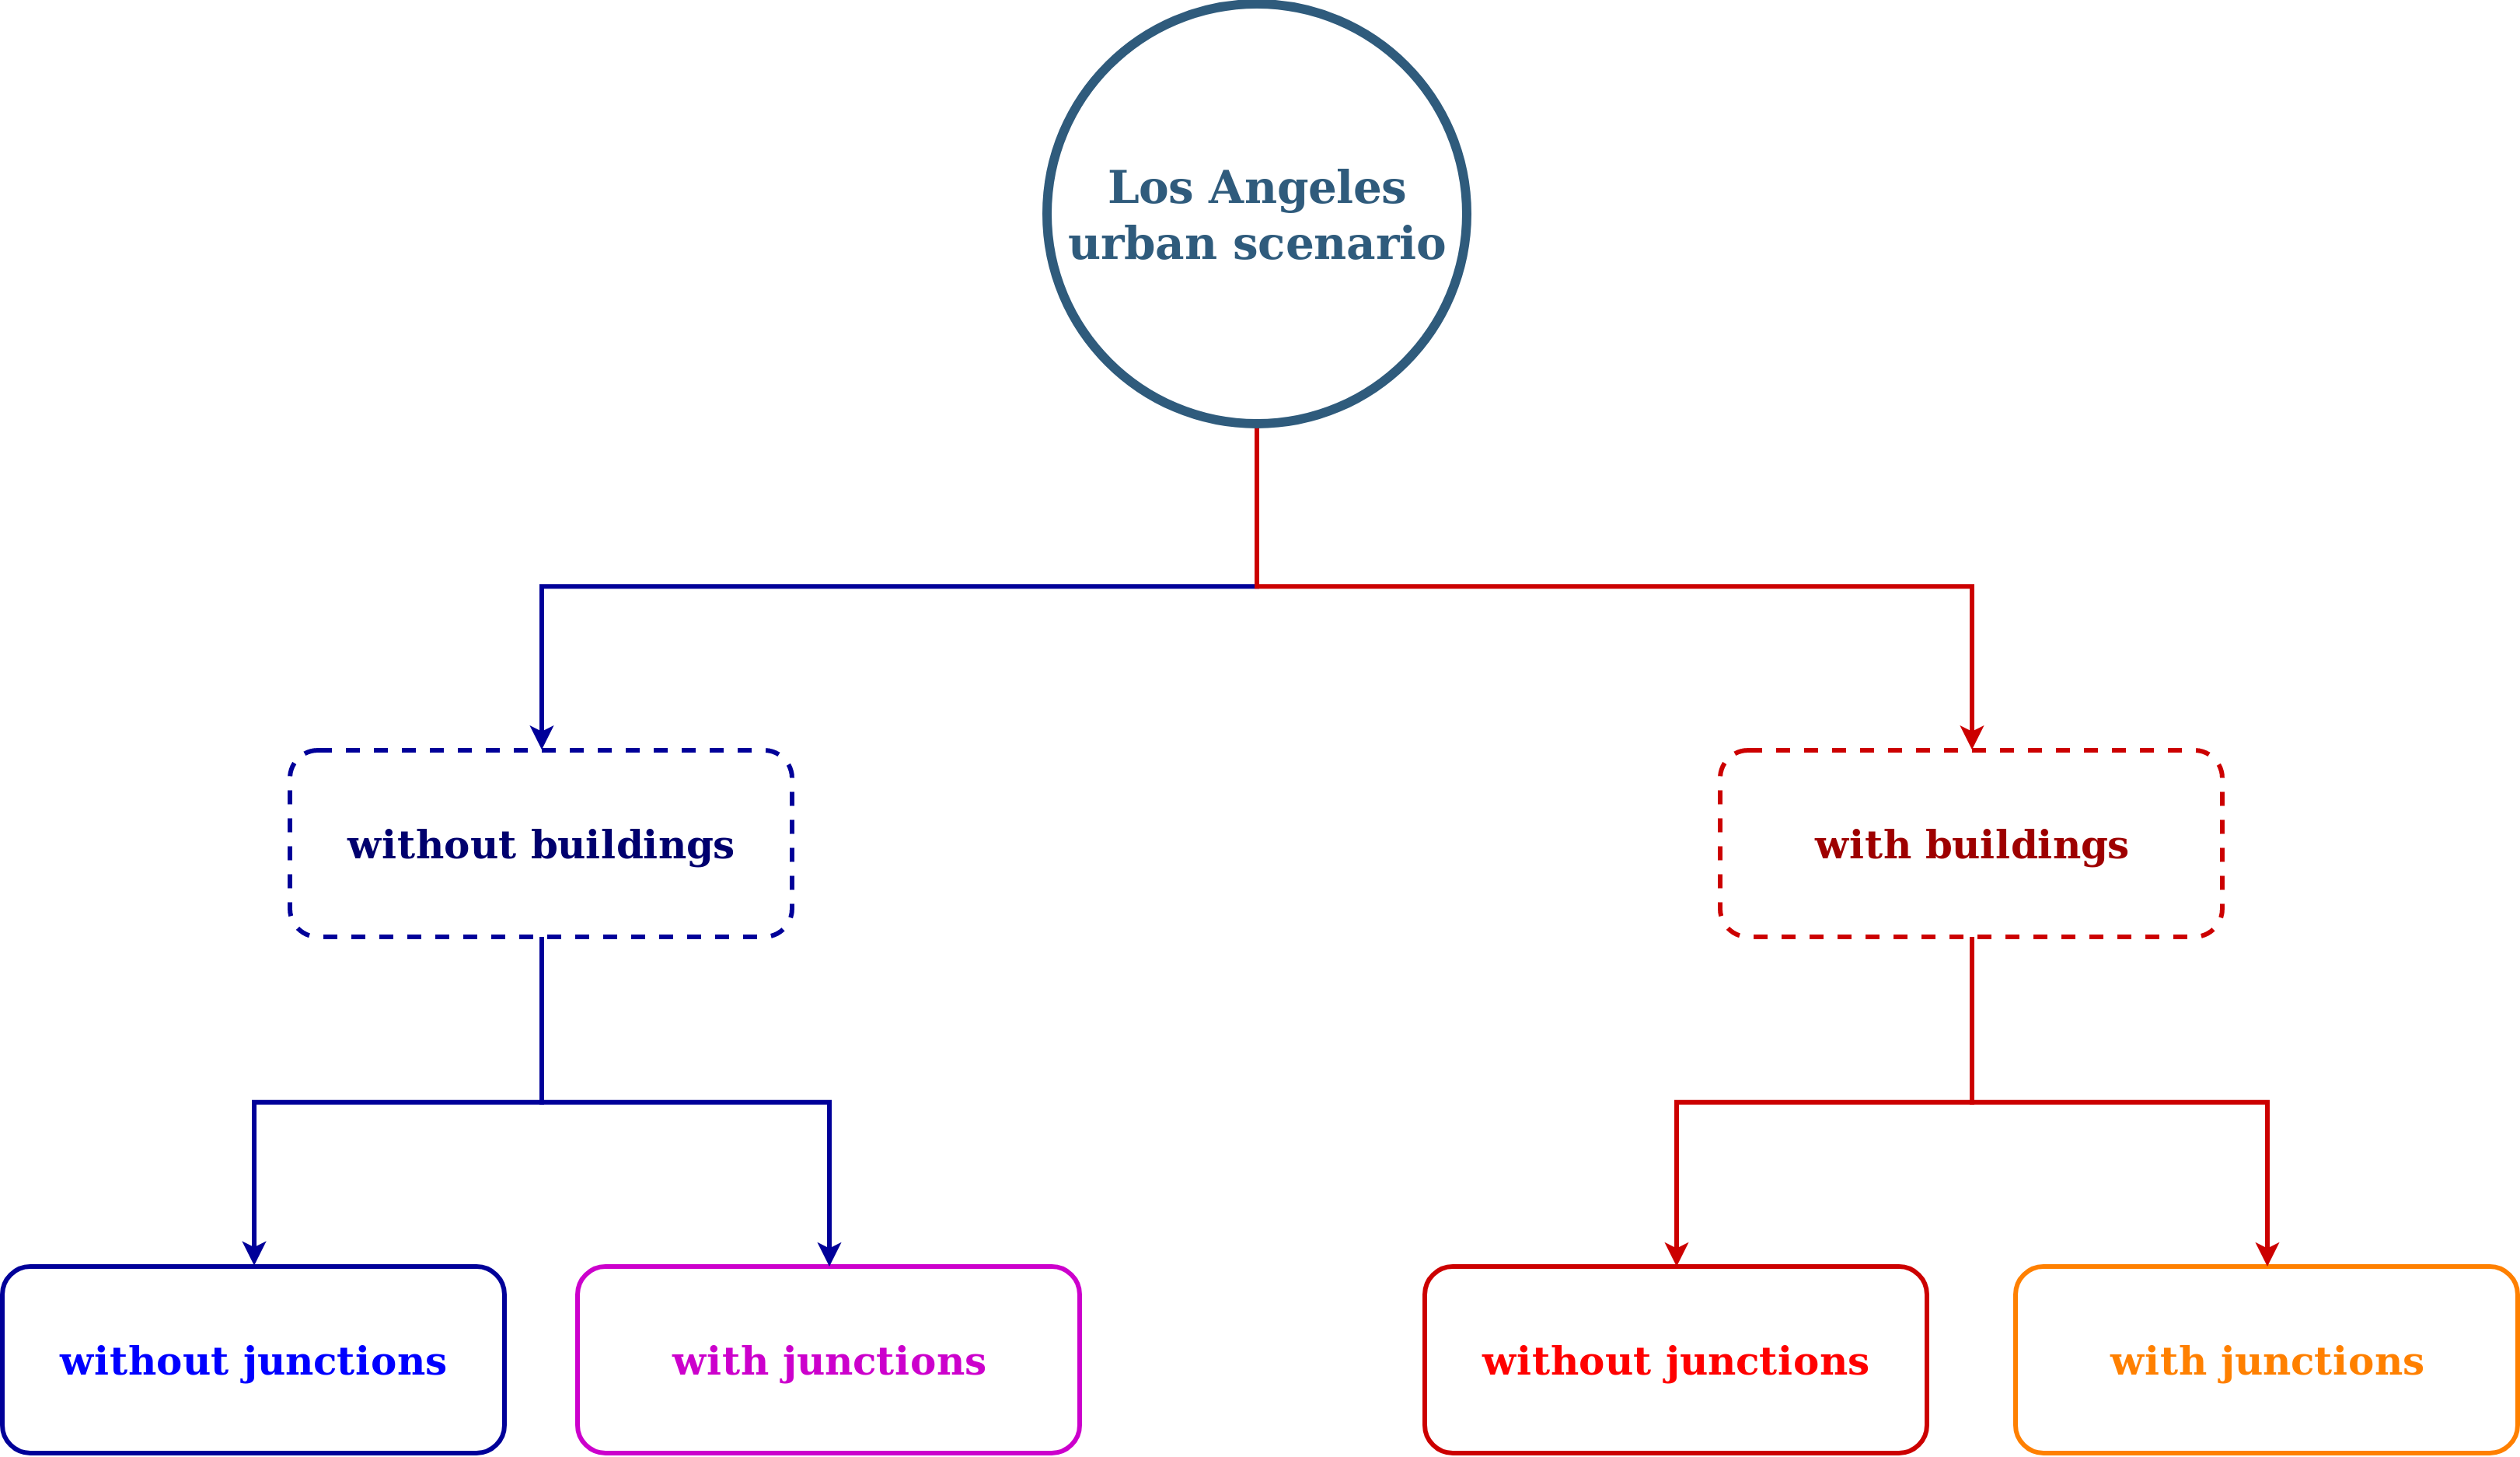
\includegraphics[width=1.0\textwidth]{immagini/la-25/overview}
			\caption{Los Angeles urban scenario test overview}
			\label{fig:la-overview}
		\end{figure}
	
		\begin{table}[H]
			\def\arraystretch{1.1}
			\rowcolors{2}{D}{P}	
			\begin{tabularx}{\textwidth}{l | l  l}
				\rowcolor{I} {\large \textcolor{white}{Parameter}} & {\large \textcolor{white}{Value}} & {\large \textcolor{white}{}} \TBstrut  \\
				\toprule
				\endhead
				%			\midrule[1pt]
				\rowcolor{P} \multicolumn{3}{c}{Scenario configuration} \\
				\midrule[1pt]
				Latitude N								& 33.9654				& \textdegree		\\
				Latitude S								& 33.9478				& \textdegree		\\
				Longitude W								& -118.3260				& \textdegree		\\
				Longitude E								& -118.3055				& \textdegree		\\
				Road length 							& 1200	 				& m		\\
				Distance between vehicles 				& 25					& m		\\
				Circumference radius					& 1000					& m		\\
				Number of vehicles						& 1465					& 		\\
				Source of alert message position		& Center				&		\\
				Number of buildings						& 8241					&		\\
				Mobility model							& ns3::ConstantPosition	&		\\
				Number of junctions						& 1288					&		\\	
				\midrule[1pt]
				\rowcolor{P} \multicolumn{3}{c}{Network configuration} \\
				\midrule[1pt]
				Shadowing model							& Obstacle Shadowing 	&		\\
				Junction modeling						& Yes					&		\\
				\midrule[1pt]
				Number of simulations per configuration	& 5000					&		\\
				\bottomrule
			\end{tabularx}
			\caption{Los Angeles urban scenario configuration}
			\label{tab:la-25}
		\end{table}
	
		\begin{figure}[H]
			\centering
			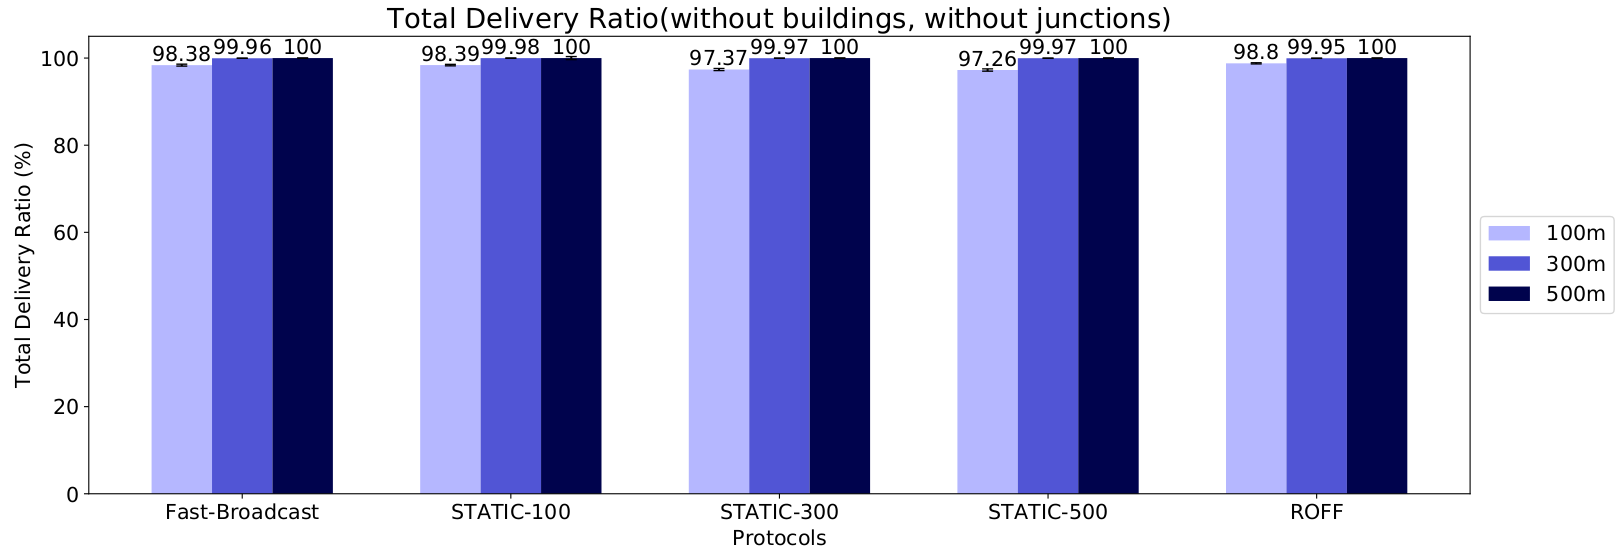
\includegraphics[width=1.0\textwidth]{immagini/la-25/b0/j0/tdr}
			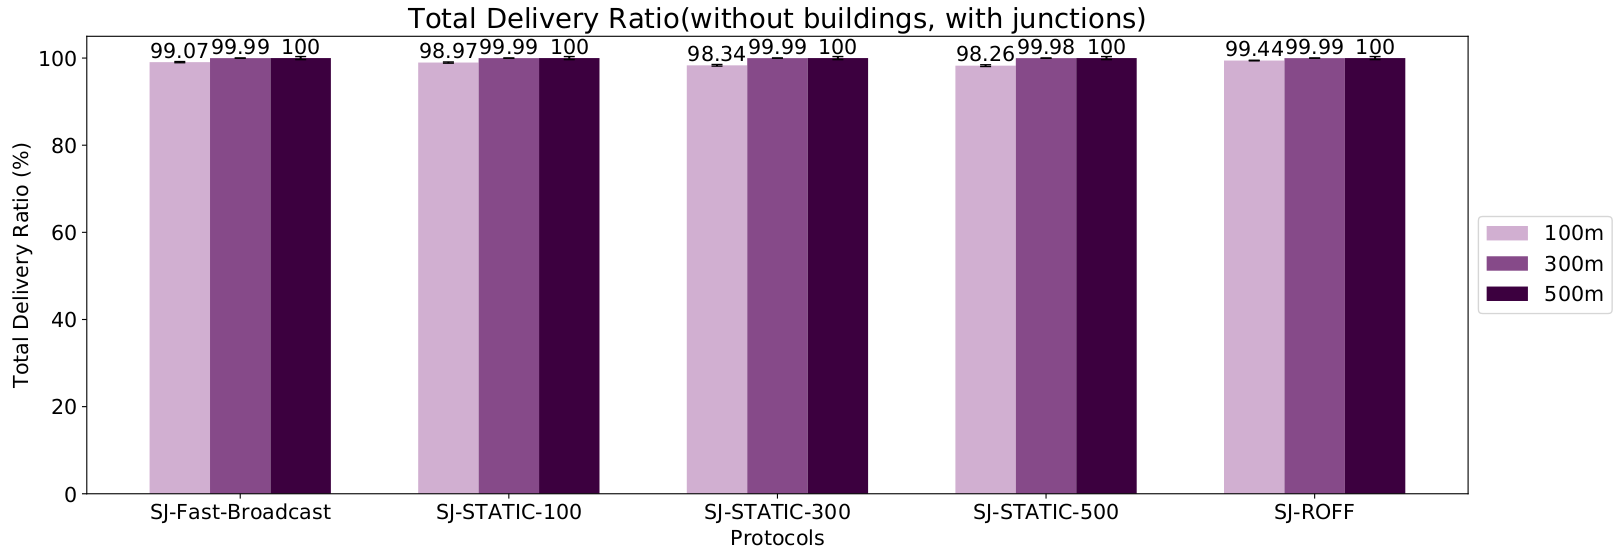
\includegraphics[width=1.0\textwidth]{immagini/la-25/b0/j1/tdr}
			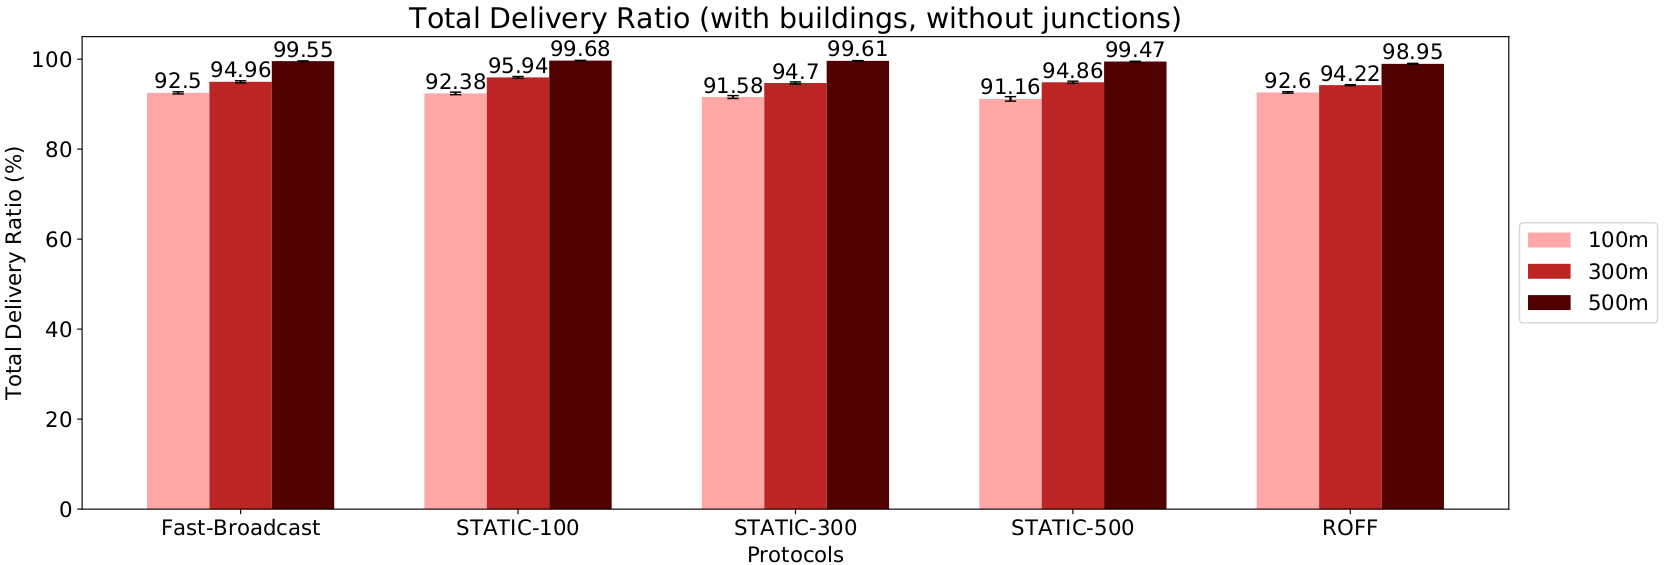
\includegraphics[width=1.0\textwidth]{immagini/la-25/b1/j0/tdr}
			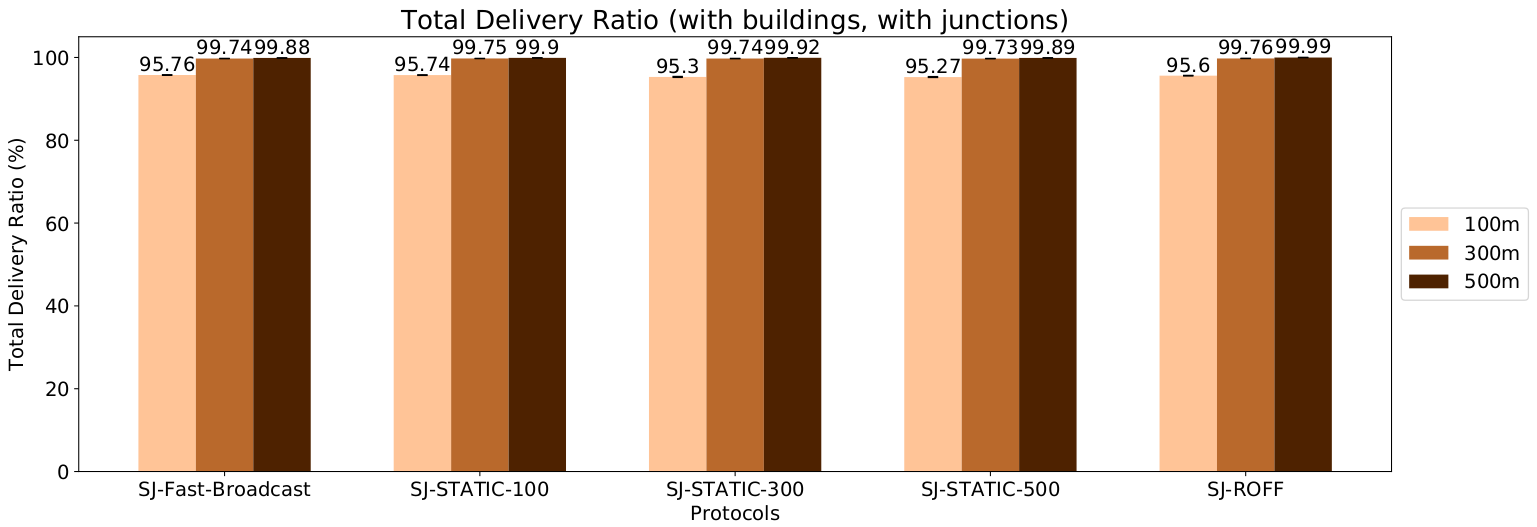
\includegraphics[width=1.0\textwidth]{immagini/la-25/b1/j1/tdr}
			\caption{\textit{TDR} for Los Angeles urban scenario}
			\label{fig:la-25-tdr}
		\end{figure}
	
		\begin{figure}[H]
			\centering
			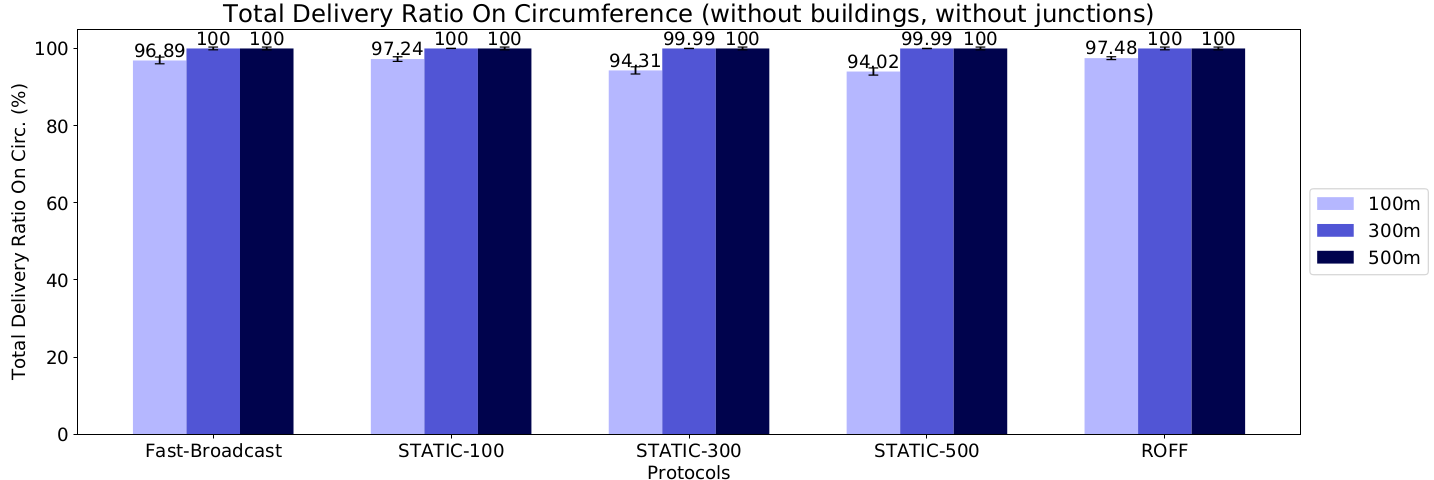
\includegraphics[width=1.0\textwidth]{immagini/la-25/b0/j0/tdroc}
			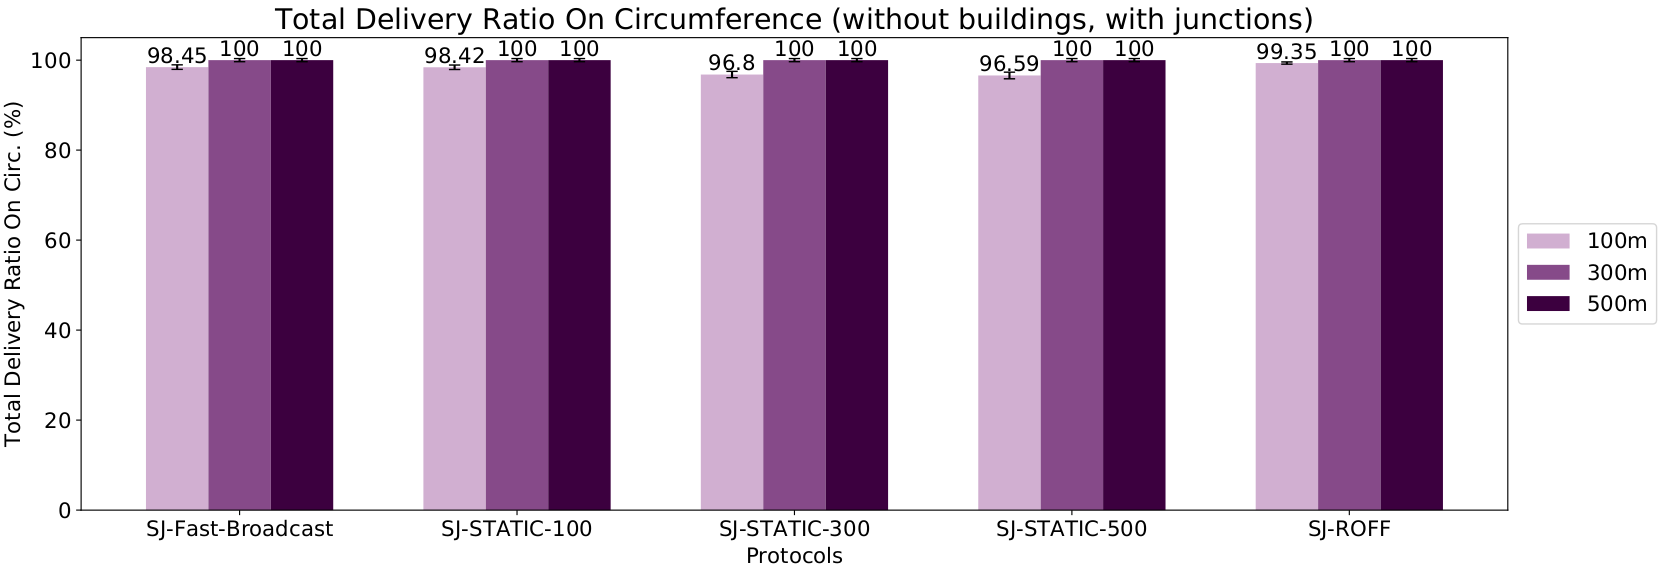
\includegraphics[width=1.0\textwidth]{immagini/la-25/b0/j1/tdroc}
			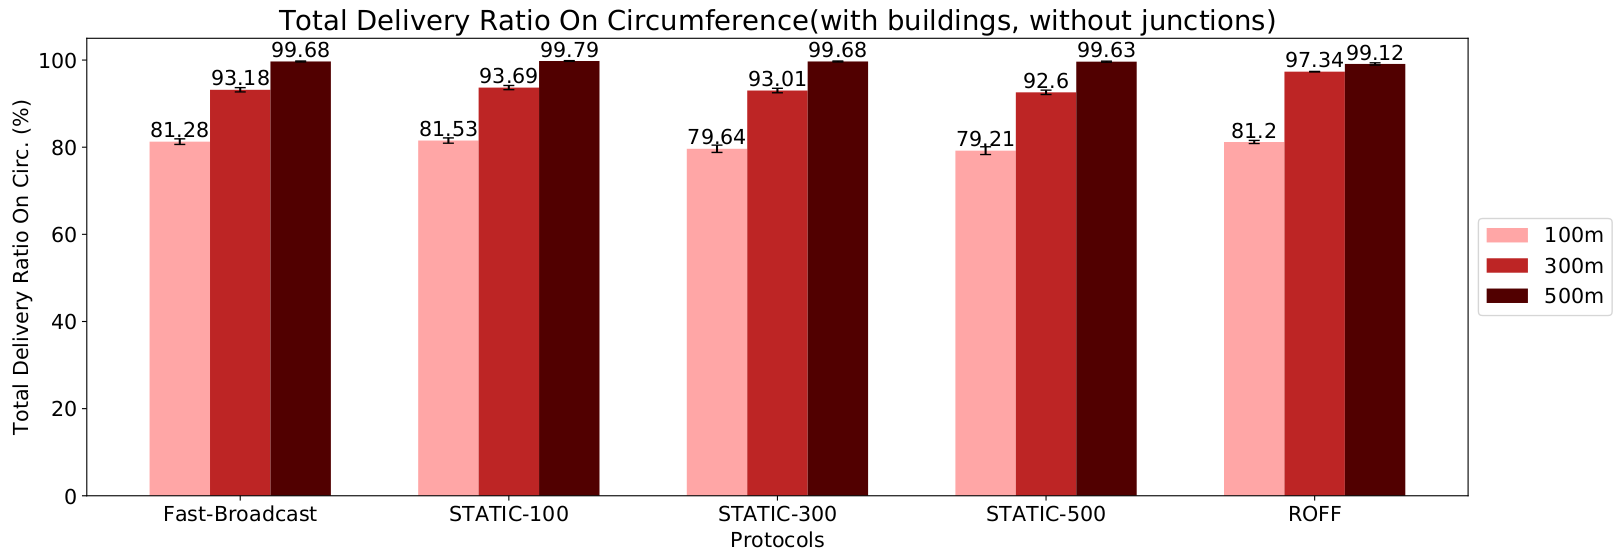
\includegraphics[width=1.0\textwidth]{immagini/la-25/b1/j0/tdroc}
			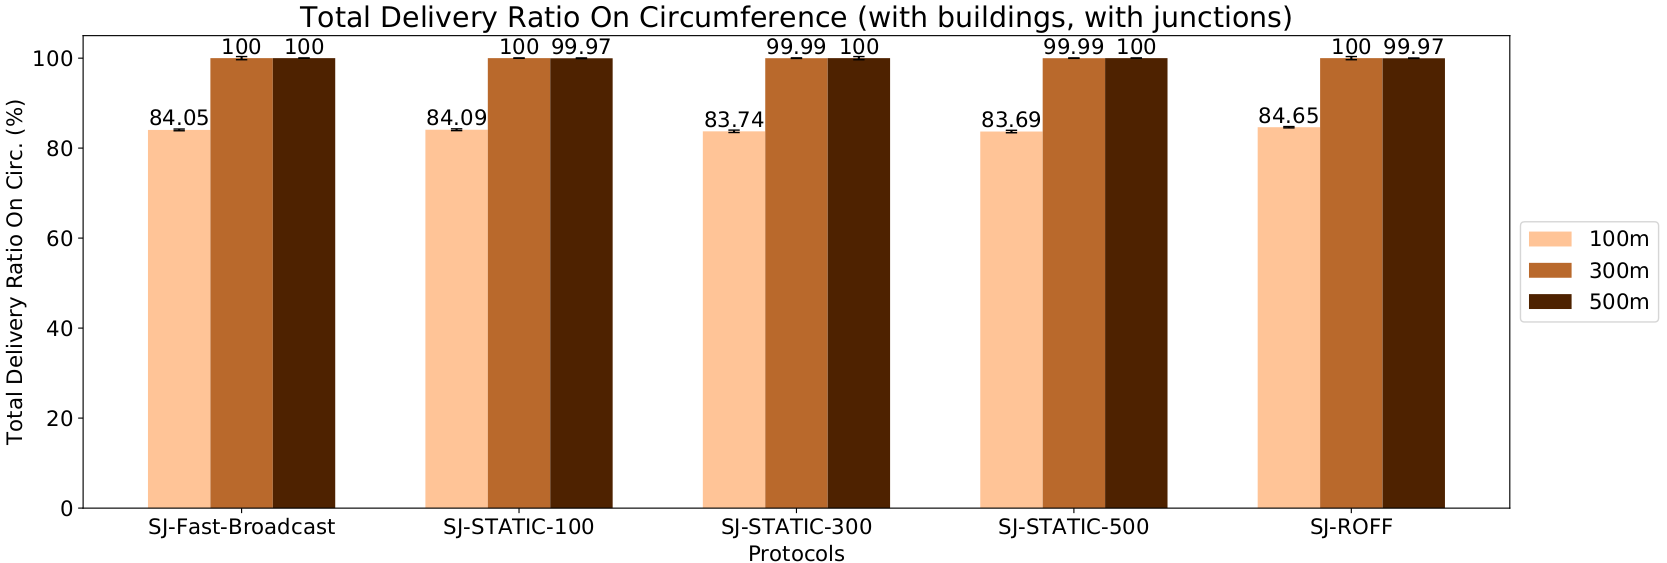
\includegraphics[width=1.0\textwidth]{immagini/la-25/b1/j1/tdroc}
			\caption{\textit{TDROC} for Los Angeles urban scenario}
			\label{fig:la-25-tdroc}
		\end{figure}

		\begin{figure}[H]
			\centering
			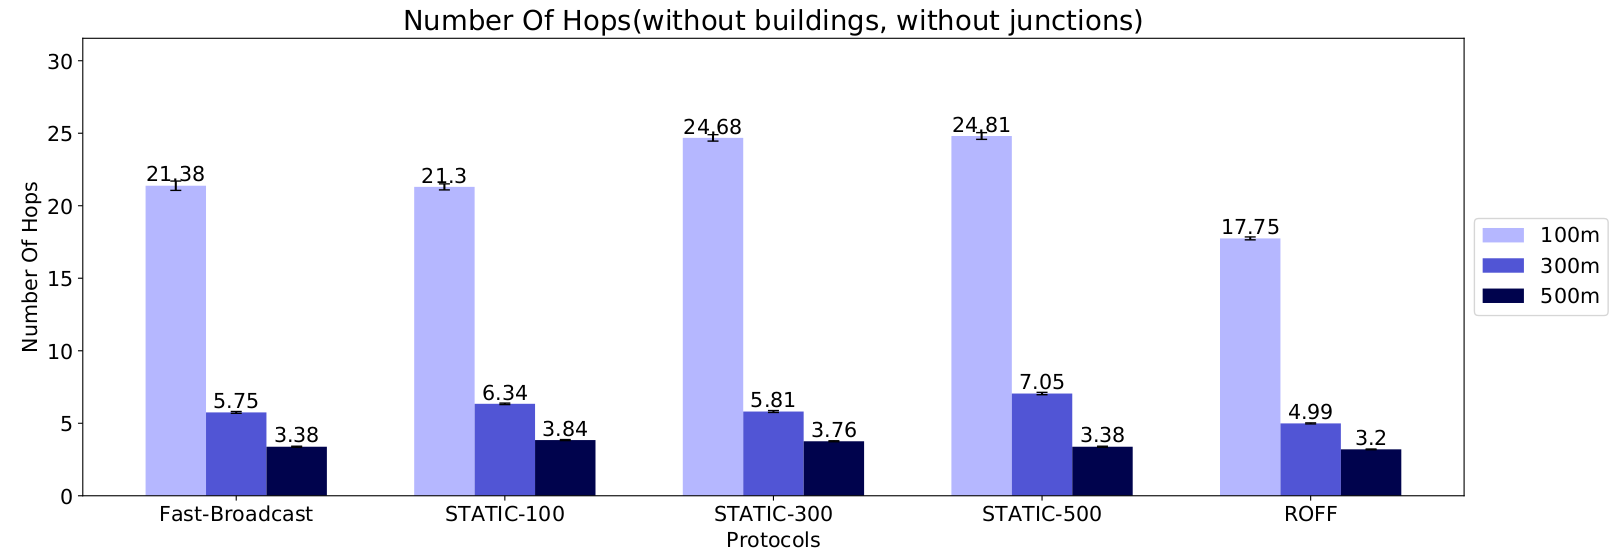
\includegraphics[width=1.0\textwidth]{immagini/la-25/b0/j0/noh}
			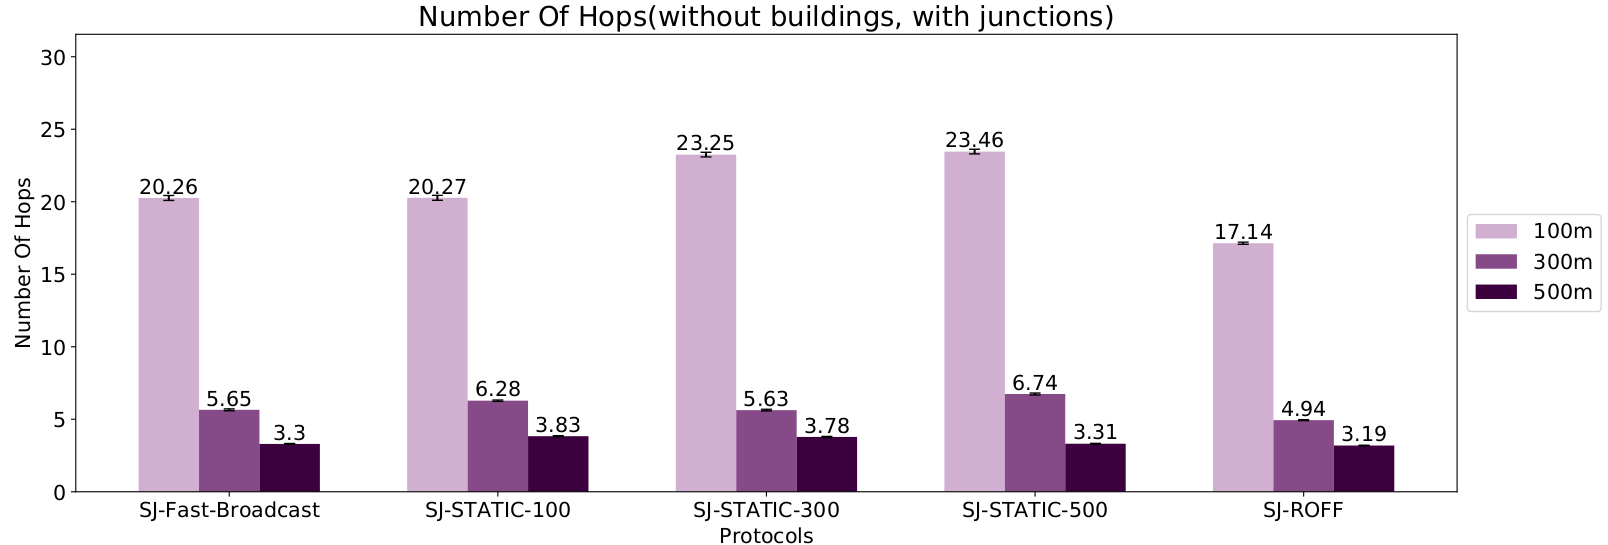
\includegraphics[width=1.0\textwidth]{immagini/la-25/b0/j1/noh}
			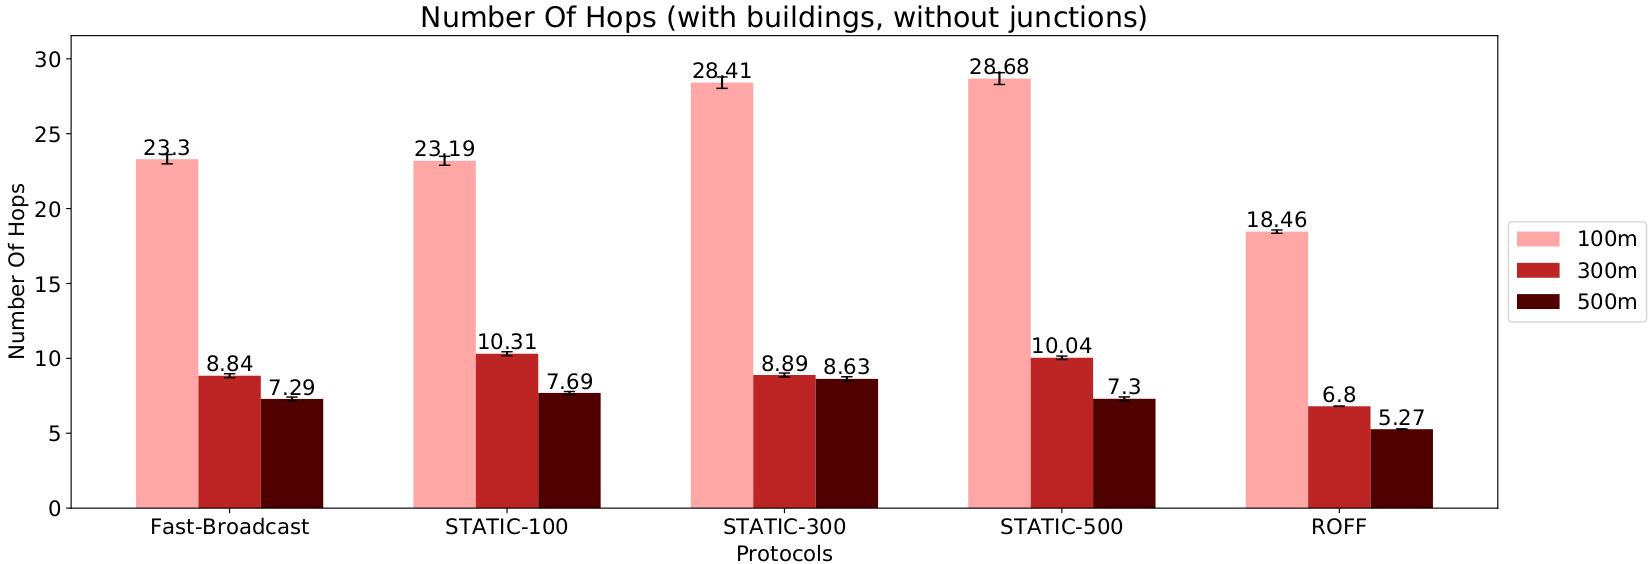
\includegraphics[width=1.0\textwidth]{immagini/la-25/b1/j0/noh}
			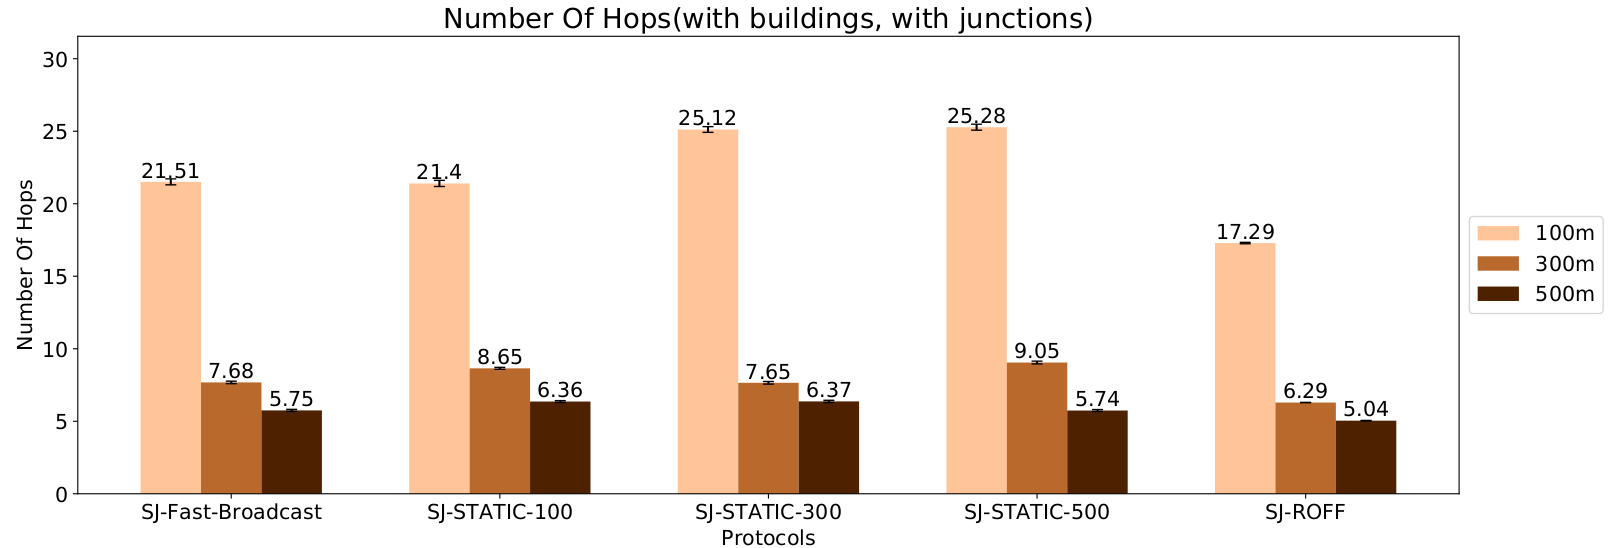
\includegraphics[width=1.0\textwidth]{immagini/la-25/b1/j1/noh}
			\caption{\textit{NOH} for Los Angeles urban scenario}
			\label{fig:la-25-noh}
		\end{figure}

		\begin{figure}[H]
			\centering
			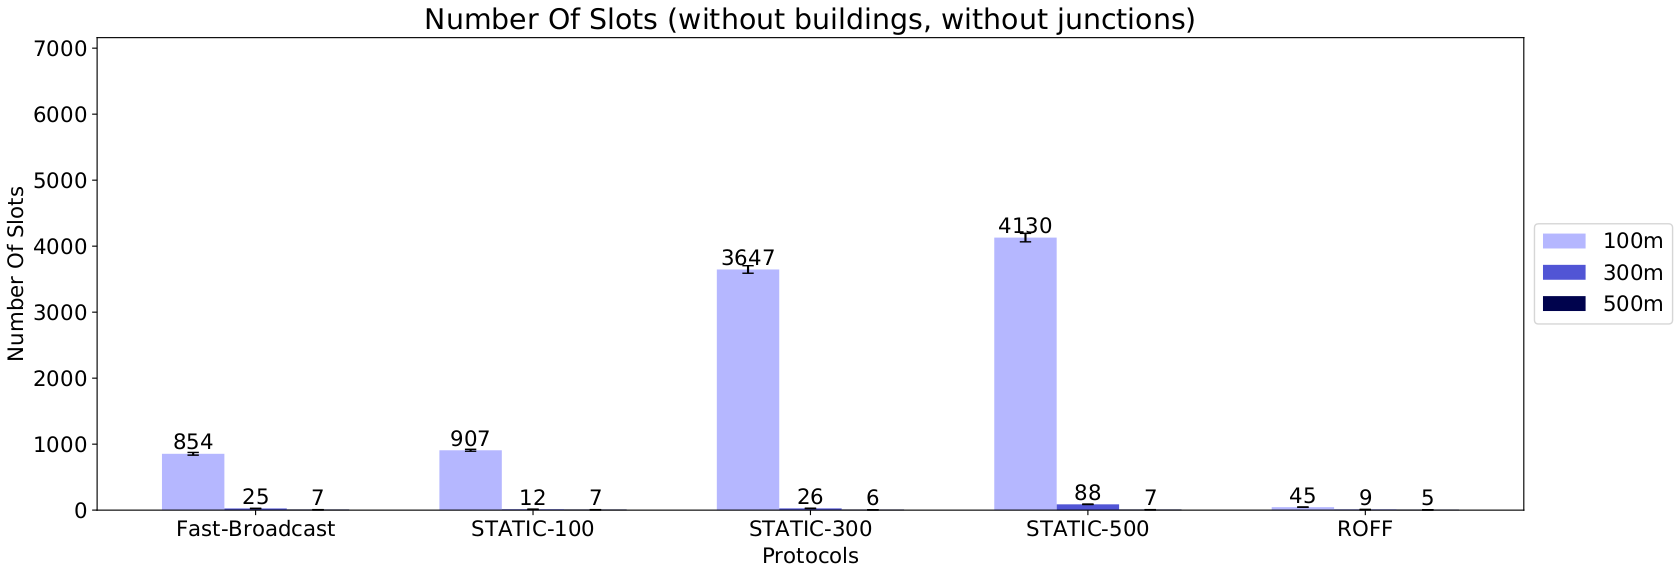
\includegraphics[width=1.0\textwidth]{immagini/la-25/b0/j0/nos}
			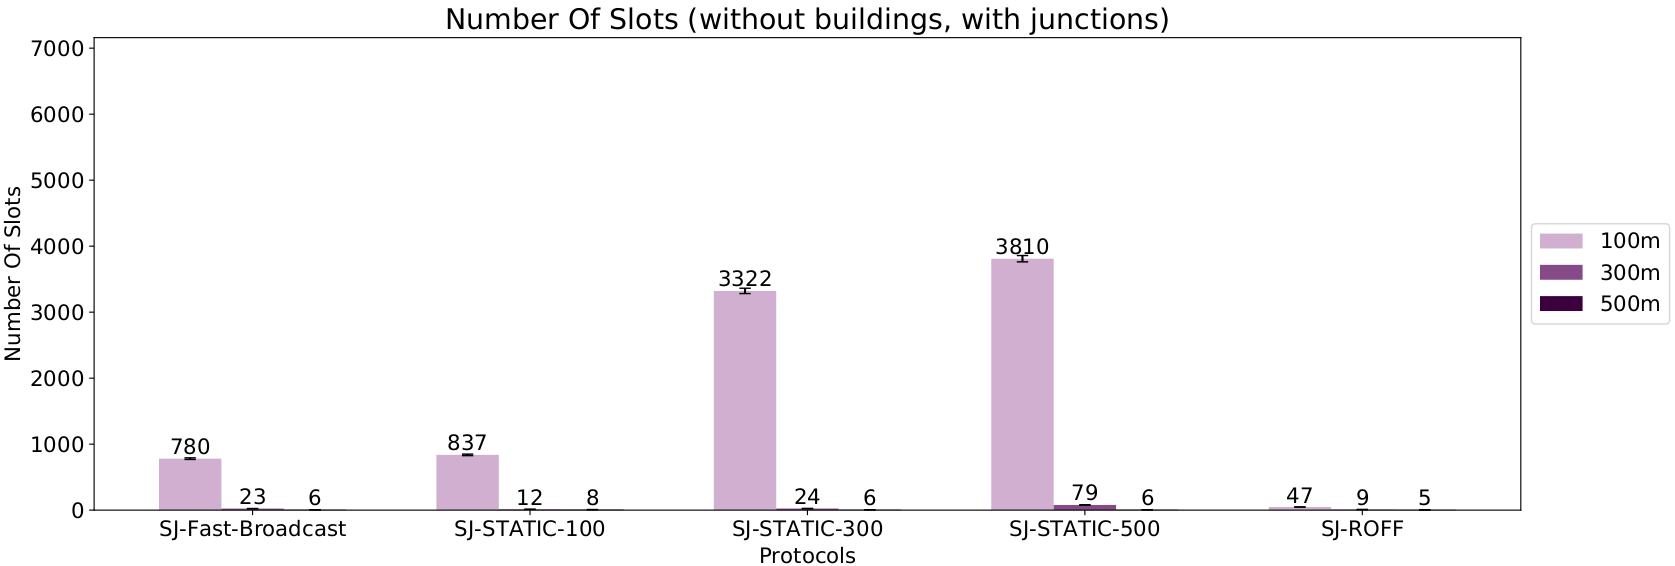
\includegraphics[width=1.0\textwidth]{immagini/la-25/b0/j1/nos}
			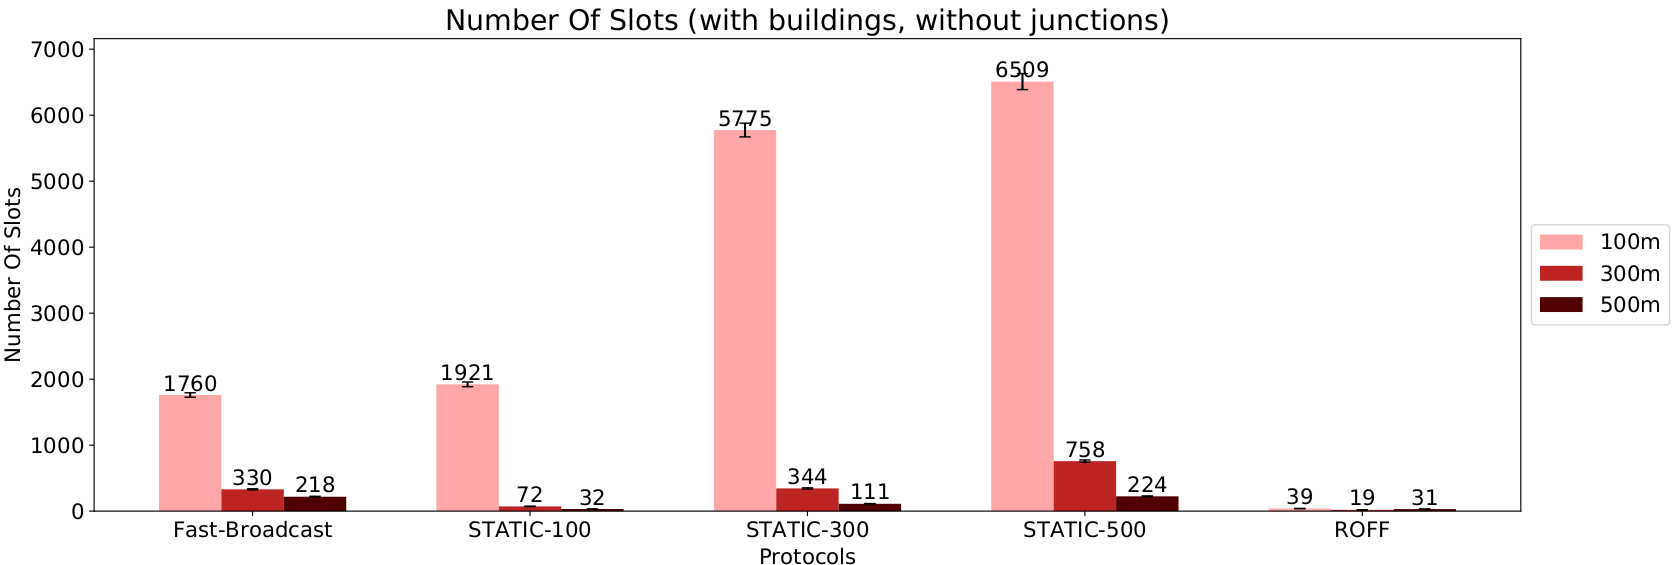
\includegraphics[width=1.0\textwidth]{immagini/la-25/b1/j0/nos}
			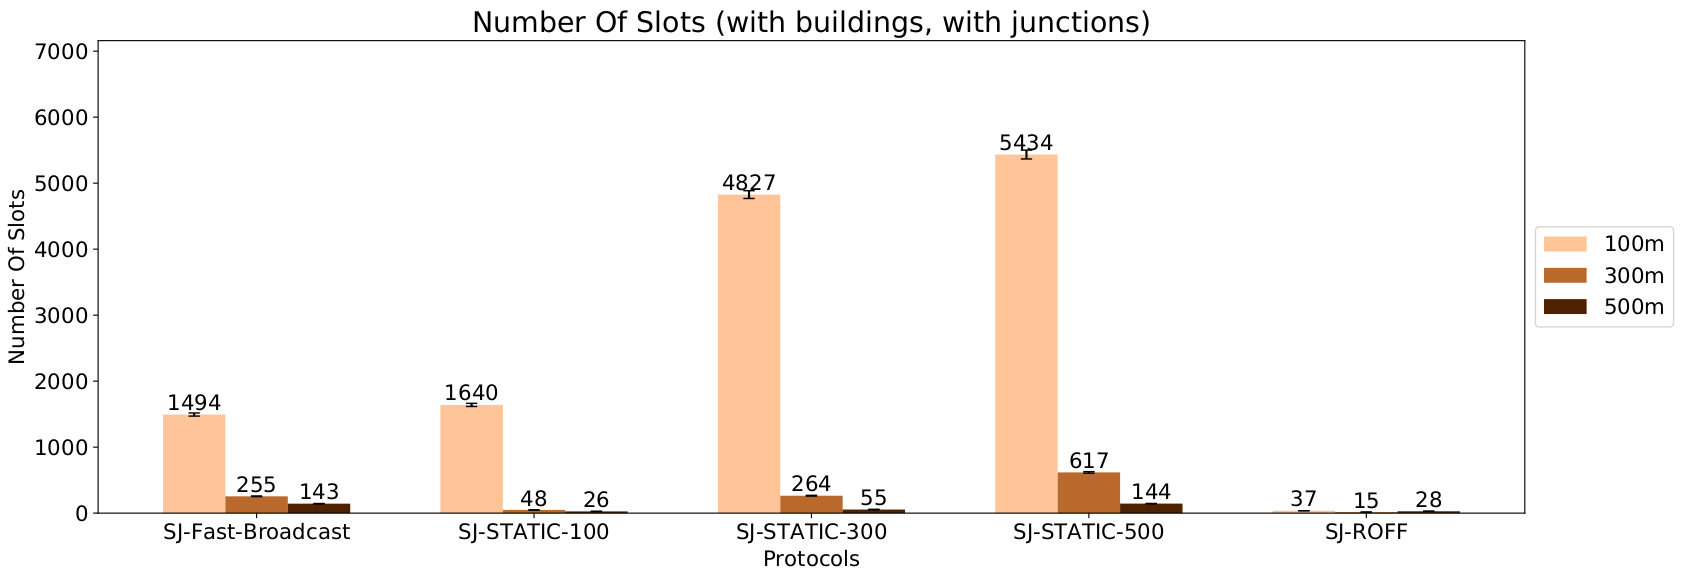
\includegraphics[width=1.0\textwidth]{immagini/la-25/b1/j1/nos}
			\caption{\textit{NOS} for Los Angeles urban scenario}
			\label{fig:la-25-nos}
		\end{figure}

		\begin{figure}[H]
			\centering
			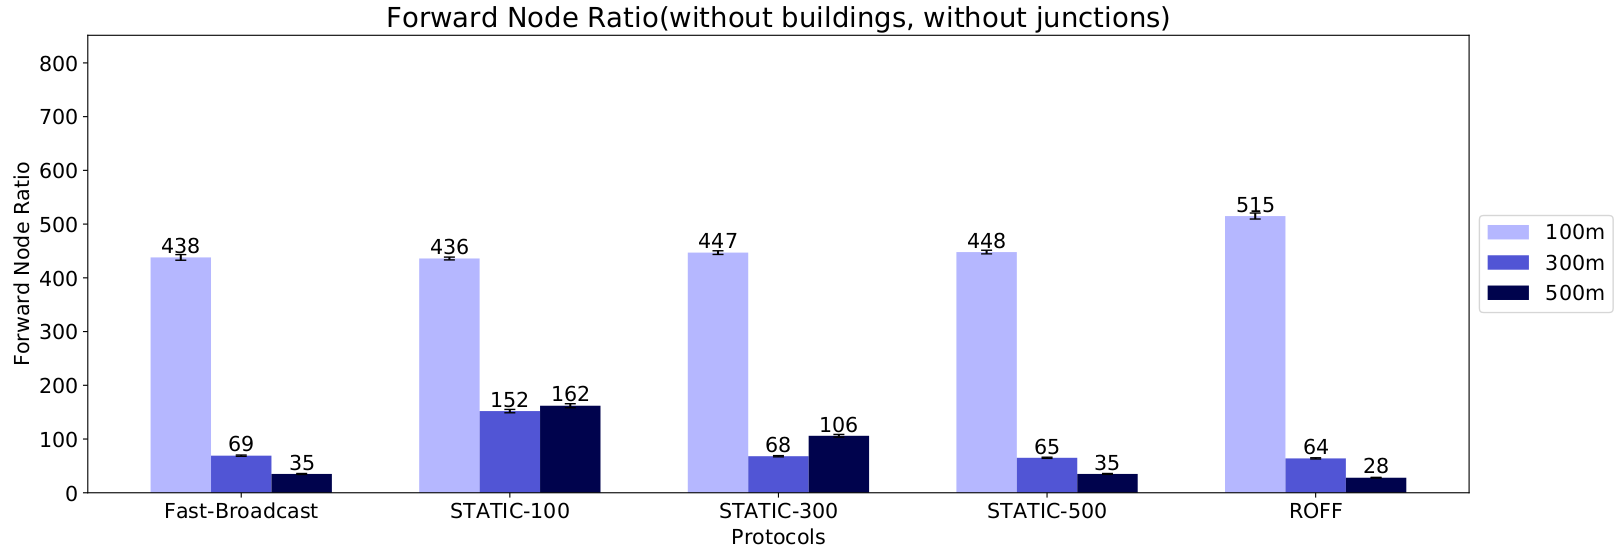
\includegraphics[width=1.0\textwidth]{immagini/la-25/b0/j0/fnn}
			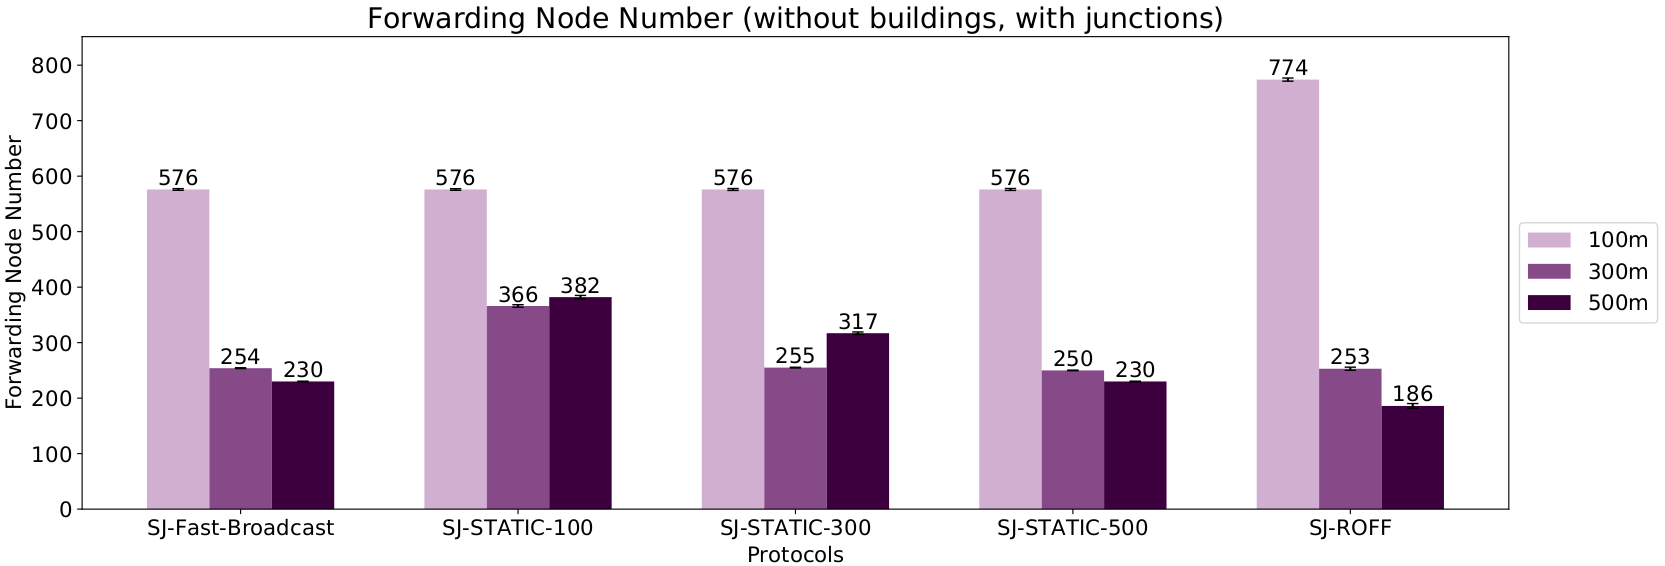
\includegraphics[width=1.0\textwidth]{immagini/la-25/b0/j1/fnn}
			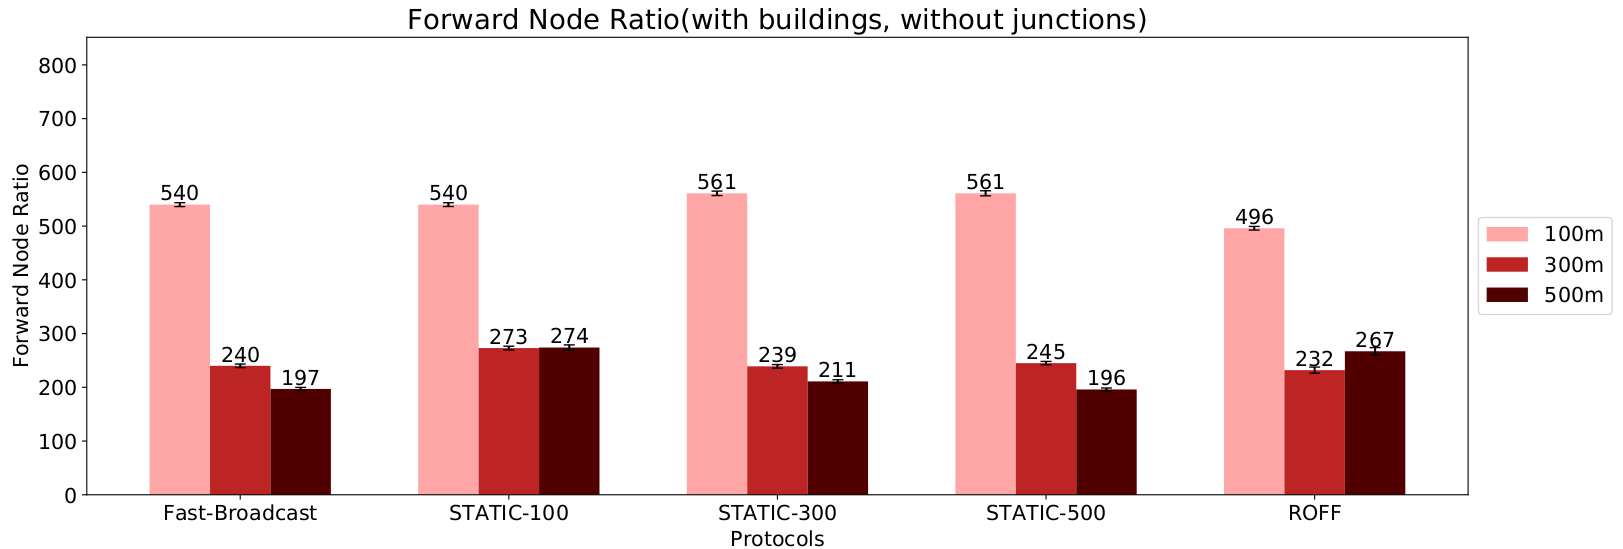
\includegraphics[width=1.0\textwidth]{immagini/la-25/b1/j0/fnn}
			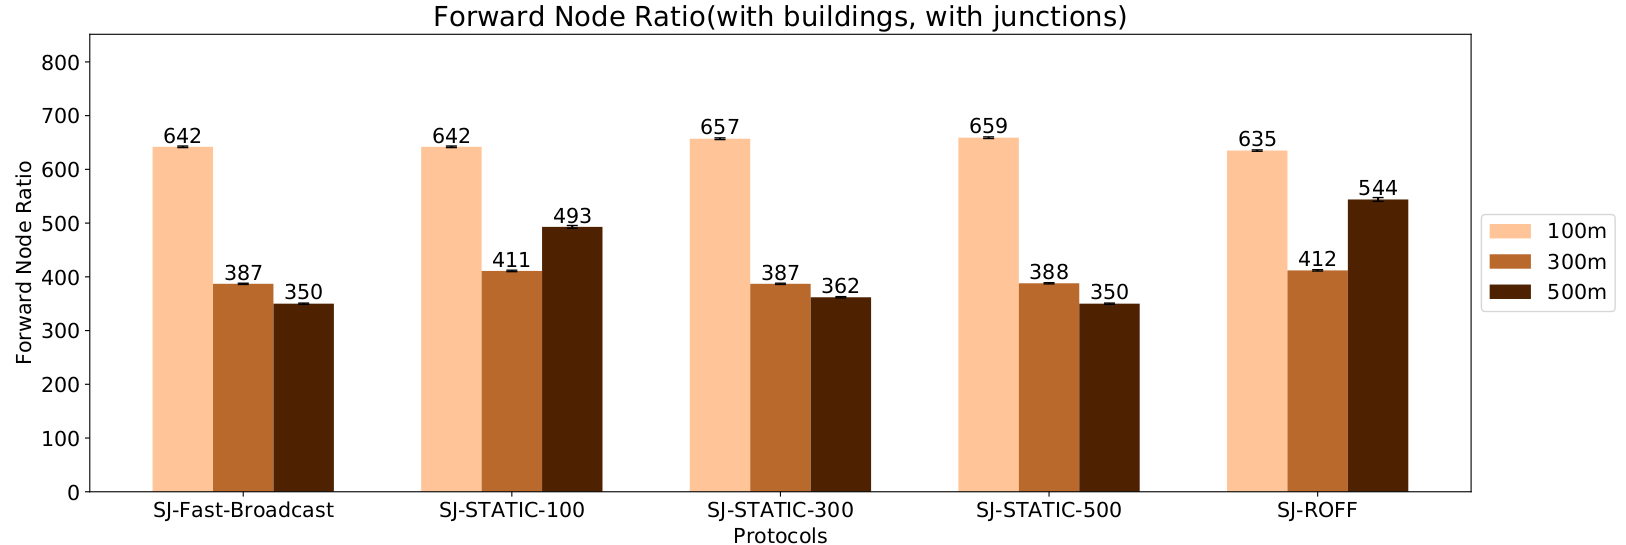
\includegraphics[width=1.0\textwidth]{immagini/la-25/b1/j1/fnn}
			\caption{\textit{FNN} for Los Angeles urban scenario}
			\label{fig:la-25-fnn}
		\end{figure}
	
		It is possible to observe the effects of the Obstacle Shadowing model on \textit{Total Delivery Ratio} and \textit{Total Delivery Ratio On Circumference}. The effects are pretty mild across all configurations, but are more noticeable with lower transmission ranges (100 and 300 meters). For example, introducing the shadowing model without considering junctions leads to a decrease of 5.97\% (98.38 to 92.5) in \textit{TDR} (Figure \ref{fig:la-25-tdr}) with a transmission range of 100 meters and a decrease of 5\% (99.96 to 94.96) with transmission range of 300 meters for Fast-Broadcast. Results for ROFF are comparable, with decreases of 6.28\% and 5.73\% respectively.
		
		
		The decrease in \textit{TDROC} (Figure \ref{fig:la-25-tdr}) is much more noticeable, especially for the 100 meters transmission range. The value decrease by 16.11\% for Fast-Broadcast and 16.74\% for ROFF. This means that introducing building shadowing leads to more problems when the Alert Message has to reach further distances. This phenomenon can be seen in Figure \ref{fig:la-coverage-fb100}.
		Vehicles not reached by the Alert Message are more concentrated towards the circumference instead of the center.
		
		\begin{figure}[H]
			\centering
			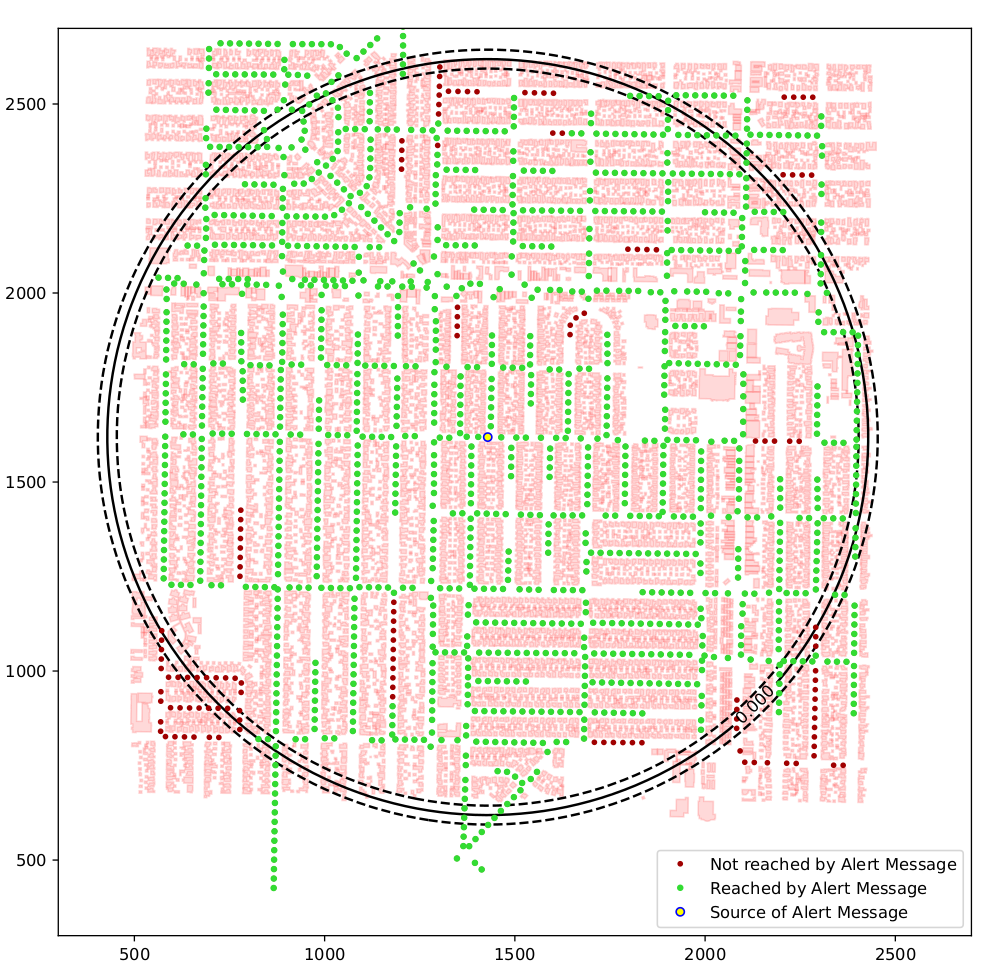
\includegraphics[width=1.0\textwidth]{immagini/la-25/la-coverage-fb100}
			\caption{Alert Message delivery for Los Angeles scenario with buildings and without junctions (Fast-Broadcast with 100 meters transmission range)}
			\label{fig:la-coverage-fb100}
		\end{figure}
		
		The introduction of the smart junction variants of the algorithms proves to be fairly effective, increasing \textit{TDR} by 3,52\% and 5,03\% when employing SJ-Fast-Broadcast instead of Fast-Broadcast for the scenario with buildings and transmission range of 100 and 300 meters respectively. Increases of the same magnitude can be noticed when utilizing SJ-ROFF instead of ROFF. With regards to \textit{TDROC}, both SJ-Fast-Broadcast and SJ-ROFF reach 100\% for 300 and 500 meters transmission ranges, while having a mild increase of around 3,40\% for 100 meters transmission range.
		
		
		Considering the Number Of Hops to reach the circumference (\ref{fig:la-25-noh}), we can observe that the introduction of the shadowing model leads to an increase in the metric's value across all algorithms. Comparing the first and third configuration, \textit{NOH} rises by 8.98, 53,74 and 115,68\% for Fast-Broadcast, and by 3.85, 36.27 and 64.69\% for ROFF, for the three increasing transmission ranges. We notice that:
		\begin{enumerate}
			\item the rise increases with the increase in transmission range;
			\item Fast-Broadcast is affected in a greater way by the shadowing model compared to ROFF.
		\end{enumerate}
		The first point is expected, since the one-hop progress is greater in a scenario with a higher transmission range. This leads to a greater probability for the signal to run into a building. In a scenario with a lower transmission range, transmissions have a lower probability to run into a building and follow more closely the road segment even without the effects of buildings. Hence, they are less likely to be influenced by the model. The second point may be due to the fact that the Neighbor Table continues to work well to identify the FFC along the road segment, leading to a smaller increase in the number of hops.
		
		
		SJ-Fast-Broadcast and SJ-ROFF need less hops in order to reach the circumference than their counterparts which do not take junctions into consideration. This holds true for both scenarios with and without buildings. This is probably due to the additional transmissions inside junctions, which help to propagate the signal along road segments in a linear way, hence covering more space with each hop. SJ-ROFF performs better than SJ-Fast-Broadcast with regards to \textit{NOH}. The difference between the two algorithms decreases as the transmission range increases.
		
		
		Regarding \textit{NOS} (Figure \ref{fig:la-25-nos}), Fast-Broadcast results increase by 106.09, 1220 and 3014\% while ROFF's ones increase by 111.11 and 520\% for 300 and 500 meters transmission range, and decrease by 4.44\% for 100 meters transmission range, when going from a building-less scenario to a scenario with buildings. Moreover, Fast-Broadcast's values are 4412.82, 1636.84 and 603.23\% higher than ROFF's values in the scenario with buildings. This goes to show the effect of empty space distribution on waiting times (here represented by the number of slots waited): when the distance between the FFC and the previous forwarder is close to the estimated transmission range, then Fast-Broadcast's waiting slots are pretty close to the minimum. But when obstacles are introduced, there might not be any PFC close to the estimated transmission range. Hence, the FFC will wait a very long time. ROFF is not affected by this phenomenon thanks to the forwarding priority acquisition, as introduced in Chapter \ref{chapter:roff}. Comparing the third and fourth image in Figure \ref{fig:la-25-nos}, we can see that the introduction of junctions is beneficial for both algorithms, leading to a decrease in \textit{NOS}. This is a consequence of the abovementioned decrease in Number Of Hops.
		
	%	todo mettere immagine dove mostriamo che a m=75 con txRange di 100 ROFF aspetta 0 mentre FB aspetta tanto?
			
		Concerning the Forwarding Node Number (Figure \ref{fig:la-25-fnn}), the value increases when the shadowing model is introduced. ROFF with 100 meters transmission range is the only configuration where the values decreases. This configuration needs further testing in order to be explained.
		The introduction of junctions brings about an increase in the number of forwardings for all algorithms, as expected. Focusing on the fourth image of Figure \ref{fig:la-25-fnn}, SJ-ROFF is affected greatly by this increase, almost equalling SJ-Fast-Broadcast with 100 meters transmission range, and with \textit{FNN} much greater values in 300 and 500 meters transmission range configurations. This might be caused by the introduction of transmissions inside junctions, which exacerbate the collision problem already reported in the previous section (Figure \ref{fig:2d-roff}), leading to an imperfect suppression of scheduled transmissions. The problem is not as severe as in the Grid scenario since the node distribution is less regular, but overall Fast-Broadcast performs slightly better in terms of FNN.
	
	\section{Padua urban scenario}
		As reported in the previous section the Los Angeles scenario, despite being realistic, still had a certain degree of regularity for what concerns vehicle distribution and scenario topology. In fact, roads and sidewalks are pretty large and the overall road positioning resembles a Grid scenario. The next step in testing consisted in employing the algorithms in a more difficult scenario, with narrower roads and intersections, smaller (if any) sidewalks and pedestrian zones where no traffic is allowed. The chosen scenario is located in Padua and, as the previous one, data about the scenario have been retrieved by OSM and processed through SUMO. The scenario is depicted in Figure \ref{fig:padua-scenario}, while its configuration is reported in Table \ref{tab:padua-25}. 
	
		\begin{figure}[H]
			\centering
			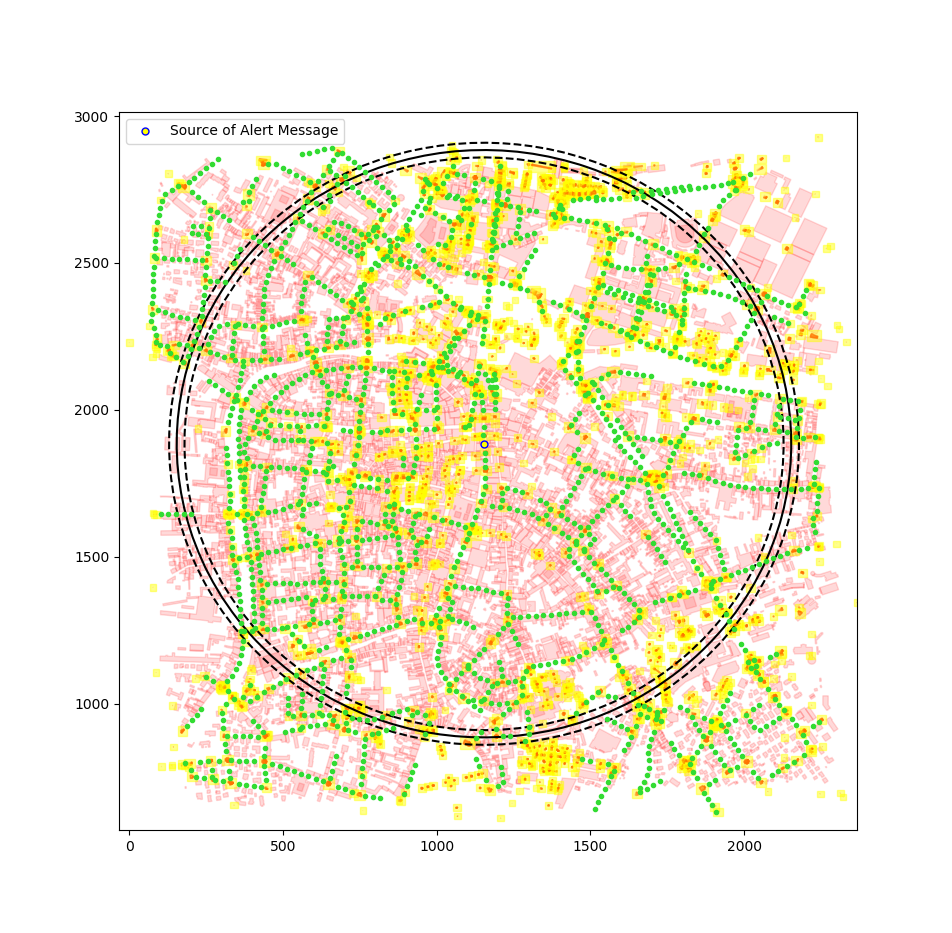
\includegraphics[width=1.0\textwidth]{immagini/padua-25/padua-scenario}
			\caption{Padua urban scenario depiction}
			\label{fig:padua-scenario}
		\end{figure}
	
		\begin{table}[H]
			\def\arraystretch{1.1}
			\rowcolors{2}{D}{P}	
			\begin{tabularx}{\textwidth}{l | l  l}
				\rowcolor{I} {\large \textcolor{white}{Parameter}} & {\large \textcolor{white}{Value}} & {\large \textcolor{white}{}} \TBstrut  \\
				\toprule
				\endhead
				%			\midrule[1pt]
				\rowcolor{P} \multicolumn{3}{c}{Scenario configuration} \\
				\midrule[1pt]
				Latitude N								& 45.4171				& \textdegree		\\
				Latitude S								& 45.3981				& \textdegree		\\
				Longitude W								& 11.8654				& \textdegree		\\
				Longitude E								& 11.8923				& \textdegree		\\
				Road length 							& 1200	 				& m		\\
				Distance between vehicles 				& 25					& m		\\
				Circumference radius					& 1000					& m		\\
				Number of vehicles						& 1775					& 		\\
				Source of alert message position		& Center				&		\\
				Number of buildings						& 6322					&		\\
				Mobility model							& ns3::ConstantPosition	&		\\
				Number of junctions						& 3231					&		\\	
				\midrule[1pt]
				\rowcolor{P} \multicolumn{3}{c}{Network configuration} \\
				\midrule[1pt]
				Shadowing model							& Obstacle Shadowing 	&		\\
				Junction modeling						& Yes					&		\\
				\midrule[1pt]
				Number of simulations per configuration	& 5000					&		\\
				\bottomrule
			\end{tabularx}
			\caption{Los Angeles urban scenario configuration}
			\label{tab:padua-25}
		\end{table}

	\section{Los Angeles smart city scenario}
		After the comparison of the algorithms in 2D scenarios, we wanted to test them in a mixed 2D-3D scenario, where drones were also employed. Drones are utilized in many military and civil applications, such as agriculture, environmental protection and traffic flow control. It is foreseeable that they will also be a part of the development of the so called "smart cities", defined as "the use of discrete new technology applications such as RFID and Internet Of Things through more holistic conception of intelligent, integrated working that is closely linked to the concept of living and user generated services"\cite{smartCity}. One of the possible applications of drones in a urban scenario could make them help vehicles in Emergency Message Dissemination in order to exploit their greater field of view and bypass the effects of ground level shadowing and obstacles. 
		
		
		This scenario is built upon the Los Angeles urban scenario presented in Section \ref{sec:la-scenario}. Two layers of drones were added to the ground level of vehicles: 
		\begin{itemize}
			\item the first layer is situated at a height of 30 meters from ground level and employs 732 drones;
			\item the second layer, employing the same number of drones, is situated at a height of 60 meters.
		\end{itemize}
		Drones are more spaced from one another than vehicles, with an average distance of 50 meters. We also wanted to test the effects of the Obstacle Model on drones in this scenario. Since the maximum height of a building in the data retrieved from OpenStreetMap is 21.9 meters, drones would not have their line of sight affected by the obstacles. Hence, as an additional configuration of this scenario, all buildings have been heightened to be taller than the second layer of drones (e.g. every building is high 100 meters).
		
		
		The TDR metric considers delivery to all entities in the scenario (both vehicles and drones), while the circumference relative to the area of interest continues to be defined in the same way as the 2D Los Angeles urban scenario, hence TDROC concerns exclusively vehicles.
		
		
		All configurations are reported in Figure \ref{fig:la-smart-city-overview}, whose colors will guide the following graph results. Table \ref{tab:la-smart-city} reports all the scenario settings.
		
		\begin{figure}[H]
			\centering
			\includegraphics[width=1.0\textwidth]{immagini/la-smart-city/overview}
			\caption{Test overview of Los Angeles smart city scenario}
			\label{fig:la-smart-city-overview}
		\end{figure}
		
	\begin{table}[H]
		\def\arraystretch{1.1}
		\rowcolors{2}{D}{P}	
		\begin{tabularx}{\textwidth}{l | l  l}
			\rowcolor{I} {\large \textcolor{white}{Parameter}} & {\large \textcolor{white}{Value}} & {\large \textcolor{white}{}} \TBstrut  \\
			\toprule
			\endhead
			%			\midrule[1pt]
			\rowcolor{P} \multicolumn{3}{c}{Scenario configuration} \\
			\midrule[1pt]
			Circumference radius					& 1000					& m		\\
			Number of vehicles						& 1465					& 		\\
			Distance between vehicles 				& 25					& m		\\
			Source of alert message position		& Center				&		\\
			Number of drone layers					& 2						&		\\
			Height of first drone layer				& 30					& m		\\
			Number of drones in first layer			& 732					& 		\\
			Height of second drone layer			& 60					& m		\\
			Number of drones in second layer		& 732					& 		\\
			Distance between drones (average)		& 50					& m		\\
			Number of buildings						& 8241					&		\\
			Building heights						& Real, 100				& m		\\
			Mobility model							& ns3::ConstantPosition	&		\\
			\midrule[1pt]
			\rowcolor{P} \multicolumn{3}{c}{Network configuration} \\
			\midrule[1pt]
			Shadowing model							& Obstacle Shadowing 	&		\\
			Junction modeling						& No					&		\\
			\midrule[1pt]
			Number of simulations per configuration	& 5000					&		\\
			\bottomrule
		\end{tabularx}
		\caption{Los Angeles urban scenario configuration}
		\label{tab:la-smart-city}
	\end{table}
	
	\section{Hello Message forging scenario}
		During our analysis we wanted to test how vulnerable the algorithms were to attacks where some malicious attacker tries to increase the end to end delay (the NOS metric in our case). The attack consists in sending fake Hello Messages to vehicles during the Estimation Phase in order to mess with their estimations. We tested two different levels of severity on the attack: a low severity one, reported in Section \ref{sec:low-severity}, and a high severity one, reported in Section \ref{sec:high-severity}. Several percentages of affected vehicles (i.e. the vehicles which receive the forged hello message bursts) ranging from 0 to 50\% have been tested. Both tests were carried out using the Los Angeles urban scenario without the effect of the Obstacle model. Only Fast-Broadcast and ROFF algorithms (and their Smart Junction variants) were tested.
		
		\subsection{Low severity attack} 
			In the low severity attack the effect of 100 different forged Hello Messages was tested. Each forged message reports a fake position such that the detected distances by the affected node (the receiver) ranges from 301 ($txRange + 1$) to 40 ($txRange + 100$). Parameters for this scenario are reported in Table \ref{tab:low-forging}.
			\label{sec:low-severity}
				\begin{table}[H]
				\def\arraystretch{1.1}
				\rowcolors{2}{D}{P}	
				\begin{tabularx}{\textwidth}{l | l  l}
					\rowcolor{I} {\large \textcolor{white}{Parameter}} & {\large \textcolor{white}{Value}} & {\large \textcolor{white}{}} \TBstrut  \\
					\toprule
					\endhead
					%			\midrule[1pt]
					\rowcolor{P} \multicolumn{3}{c}{Scenario configuration} \\
					\midrule[1pt]
					Vehicles affected by forging			& 0, 10, 20, 30, 40, 50 & \%	\\
					Number of forged messages				& 100					&		\\
					Forged distances						& 301, 302,...,400		&		\\
					\midrule[1pt]
					\rowcolor{P} \multicolumn{3}{c}{Network configuration} \\
					\midrule[1pt]
					Transmission power						& 4.6					& dBm	\\
					Transmission range						& 300					&		\\
					Shadowing model							& No					&		\\
					Junction modeling						& Yes					&		\\
					\midrule[1pt]
					Number of simulations per configuration	& 1000					&		\\
					\bottomrule
				\end{tabularx}
				\caption{High severity forging attack scenario configuration based on Los Angeles urban scenario}
				\label{tab:low-forging}
			\end{table}
		
		\subsection{High severity attack}
			In the high severity attack the number of forged Hello Messages was increased to 1000. Moreover, even the fake positions included in the messages have been increased in a way such that the receivers detected distances ranging from 10000 to 11000 meters. Parameters for this scenario are reported in Table \ref{tab:high-forging}.
			\label{sec:high-severity}
			\begin{table}[H]
				\def\arraystretch{1.1}
				\rowcolors{2}{D}{P}	
				\begin{tabularx}{\textwidth}{l | l  l}
					\rowcolor{I} {\large \textcolor{white}{Parameter}} & {\large \textcolor{white}{Value}} & {\large \textcolor{white}{}} \TBstrut  \\
					\toprule
					\endhead
					%			\midrule[1pt]
					\rowcolor{P} \multicolumn{3}{c}{Scenario configuration} \\
					\midrule[1pt]
					Vehicles affected by forging			& 0, 10, 20, 30, 40, 50 & \%	\\
					Number of forged messages				& 1000					&		\\
					Forged distances						& 10000, 10001,...,11000			&		\\
					\midrule[1pt]
					\rowcolor{P} \multicolumn{3}{c}{Network configuration} \\
					\midrule[1pt]
					Transmission power						& 4.6					& dBm	\\
					Transmission range						& 300					&		\\
					Shadowing model							& No					&		\\
					Junction modeling						& No					&		\\
					\midrule[1pt]
					Number of simulations per configuration	& 1000					&		\\
					\bottomrule
				\end{tabularx}
				\caption{High severity forging attack scenario configuration based on Los Angeles urban scenario}
				\label{tab:high-forging}
			\end{table}
			
	
	\section{Varying vehicle density scenario}
	
	\section{Contention window}
		\begin{table}[H]
			\def\arraystretch{1.1}
			\rowcolors{2}{D}{P}	
			\begin{tabularx}{\textwidth}{l | l  l}
				\rowcolor{I} {\large \textcolor{white}{Parameter}} & {\large \textcolor{white}{Value}} & {\large \textcolor{white}{}} \TBstrut  \\
				\toprule
				\endhead
				\midrule[1pt]
				\rowcolor{P} \multicolumn{3}{c}{Network configuration} \\
				\midrule[1pt]
				Shadowing model							& No					&		\\
				Junction modeling						& No					&		\\
				\midrule[1pt]
				\rowcolor{P} \multicolumn{3}{c}{Protocols configuration} \\
				\midrule[1pt]
				%			Protocols tested						& \makecell{FB, ROFF, STATIC100, \\ STATIC300, STATIC500} & \\
				FB contention window					& [16, 128], [32, 1024]	& slot	\\
				ROFF distance range (\textit{k} parameter) & 1					&		\\	
				\midrule[1pt]
				Number of simulations per configuration	& 1000					&		\\
				\bottomrule
			\end{tabularx}
			\label{table:fb-cw}
			\caption{Smaller contention window scenario configuraton based on Los Angeles urban scenario}
		\end{table}

	
	
	

%		../../scripts/graphs/out/Platoon-15km/b0/j0-cw[32-1024]/totCoverage
	